%http://pastebin.com/PxAwdRav
%http://pastebin.com/QrbRv3Dc
%http://pastebin.com/dmxhDtcS
%%%%%%%%%%%%%%%%%%%%%%%%%%%%%%%%%%%%%%%%%%%%%%%%%%%%%%%%%%%%%%%%%%%%%%
% LaTeX Example: Project Report
%
% Source: 
%tp://www.howtotex.com
%
% Feel free to distribute this example, but please keep the referral
% to howtotex.com
% Date: March 2011 
% 
%%%%%%%%%%%%%%%%%%%%%%%%%%%%%%%%%%%%%%%%%%%%%%%%%%%%%%%%%%%%%%%%%%%%%%
% How to use writeLaTeX: 
%
% You edit the source code here on the left, and the preview on the
% right shows you the result within a few seconds.
%
% Bookmark this page and share the URL with your co-authors. They can
% edit at the same time!
%
% You can upload figures, bibliographies, custom classes and
% styles using the files menu.
%
% If you're new to LaTeX, the wikibook is a great place to start:
% http://en.wikibooks.org/wiki/LaTeX
%
%%%%%%%%%%%%%%%%%%%%%%%%%%%%%%%%%%%%%%%%%%%%%%%%%%%%%%%%%%%%%%%%%%%%%%
% Edit the title below to update the display in My Documents
%\title{Project Report}
%
%%% Preamble
\documentclass[paper=a4, fontsize=11pt]{scrartcl}
\usepackage[T1]{fontenc}
\usepackage{fourier}
\usepackage{abstract}
\usepackage[english]{babel}															% English language/hyphenation
\usepackage[protrusion=true,expansion=true]{microtype}	
\usepackage{amsmath,amsfonts,amsthm} % Math packages
\usepackage[pdftex]{graphicx}	
\usepackage{url}
\usepackage{float}
\restylefloat{table}


%%% Custom sectioning
\usepackage{sectsty}
\allsectionsfont{\centering \normalfont\scshape}


%%% Custom headers/footers (fancyhdr package)
\usepackage{fancyhdr}
\pagestyle{fancyplain}
\fancyhead{}											% No page header
\fancyfoot[L]{}											% Empty 
\fancyfoot[C]{}											% Empty
\fancyfoot[R]{\thepage}									% Pagenumbering
\renewcommand{\headrulewidth}{0pt}			% Remove header underlines
\renewcommand{\footrulewidth}{0pt}				% Remove footer underlines
\setlength{\headheight}{13.6pt}


%%% Equation and float numbering
\numberwithin{equation}{section}		% Equationnumbering: section.eq#
\numberwithin{figure}{section}			% Figurenumbering: section.fig#
\numberwithin{table}{section}				% Tablenumbering: section.tab#

% % % Commands for grid graphics
\newcounter{eqn}
\renewcommand*{\theeqn}{\alph{eqn})}
\newcommand{\num}{\refstepcounter{eqn}\text{\theeqn}\;}

\makeatletter
\newcommand{\putindeepbox}[2][0.7\baselineskip]{{%
    \setbox0=\hbox{#2}%
    \setbox0=\vbox{\noindent\hsize=\wd0\unhbox0}
    \@tempdima=\dp0
    \advance\@tempdima by \ht0
    \advance\@tempdima by -#1\relax
    \dp0=\@tempdima
    \ht0=#1\relax
    \box0
}}
\makeatother

%%% Maketitle metadata
\newcommand{\horrule}[1]{\rule{\linewidth}{#1}} 	% Horizontal rule

\title{
		%\vspace{-1in} 	
		\usefont{OT1}{bch}{b}{n}
		\normalfont \normalsize \textsc{Autonomous Agents Assignment 2} \\ [25pt]
		\horrule{0.5pt} \\[0.4cm]
		\huge Single Agent Learning \\
		\horrule{2pt} \\[0.5cm]
}
\author{
		%\normalfont 								\normalsize
        Duy Chuan Ha, Said Al Faraby, Christos Louizos, Oana Munteanu %[-3pt]		%\normalsize
        \\
        \\
        \today
}
\date{}
\renewcommand{\abstractnamefont}{\normalfont\Large\bfseries}
\renewcommand{\abstracttextfont}{\normalfont\bfseries}


%%% Begin document
\begin{document}
\maketitle
\bigskip
\begin{abstract}
The aim of this assignment is to focus on the research of a learning scenario in which the agent does not know the transition probabilities, nor the reward structure. For completing that, we have implemented and tested various methods, namely  Q-learning, On-policy Monte Carlo Control, Off-policy Monte Carlo Control and Sarsa in order to explain their theoretical differences, to compare their results and to conclude which one is the optimal high-reward policy which yields from the fastest moves of the predator in order to catch the prey.\\
\end{abstract}
%\newpage
%\tableofcontents 
%\newpage

\section{Introduction}
In this research, we have considered that the model is unknown and, in this situation, two approaches can be pursued. A model-based approach tries to learn the model explicitly and then use methods like Dynamic Programming to compute the optimal policy with respect to the estimate of the model. On the other hand, a model-free approach concentrates on learning the state value function (Q-value function) directly and obtaining the optimal policy from this estimates.\\
We shall try to focus on model-free methods for learning in MDPs by making use of: \\
$\bullet$ Q-learning with $\epsilon$-greedy action selection; \\
$\bullet$ Q-learning with Softmax action selection; \\
$\bullet$ On-policy Monte-Carlo Control; \\
$\bullet$ Off-policy Monte-Carlo Control; \\
$\bullet$ Sarsa.

In this assignment, we have explored the learning methods for estimating value functions and discovering  optimal policies.\\ 
Monte Carlo methods (MC methods) require only experience through sample sequences of states, actions and rewards from on-line or simulated interaction with an environment. They do not require prior knowledge of the environment's dynamics, yet can still achieve an optimal behavior. Concerning the disadvantages of these methods, Monte Carlo method is conceptually simple and do not require any model, but is not suited for step-by-step incremental  computation.\\
Temporal-Difference Learning (TD Learning) represents a combination of Monte Carlo and Dynamic Programming ideas. Like MC methods, TD methods do not require a model, while like DP, TD methods bootstrap; they update estimates based on other learned estimates, without waiting for a final outcome like MC:
\begin{align}
V(s_t) \leftarrow V(s_t) + \alpha [R_t-V(s_t)] \qquad \text{MC: update target is $R_t$} \\
V(s_t) \leftarrow V(s_t) + \alpha[r_{t+1}+\gamma V(s_{t+1})-V(s_t)] \qquad \text{TD: update target is $r_{t+1}+\gamma V_t(s_{t+1})$}
\end{align}
During this research, the main focus is to understand better the idea of each model-free method and to highlight some demands like: What are the differences, both theoretical and practical, between all the implemented methods? Which method converges to the most optimal policy faster?\\ 


%overview of what will follow
In order to do that, we have structured the report in 4 sections comprising: section 2, where we explain the theoretical background of each method and learn how to implement the pseudo-code; in section 3 we present  some of the theoretical differences between the methods and we show the experiments through results and graphics, afterwards in section 4 we discuss about the brief conclusion of this assignment.

%\subsection{Environment: Should we keep this? Maybe the 1st paragraph?}
%\label{environment}
%The environment is a 11x11 grid which is toroidal and each state is encoded as the positions of the two agents, predator and prey.
%insert later dataflow diagram
%The simulator is defined through a while-loop of a hundred runs where the initial position of the predator is (0,0) and that of the prey (5,5). In each transition, the predator will make a move first and then the prey, according to their respective policies. Each run is composed of an episode, where the goal of the predator is to capture the prey, which can be interpreted as the end state of this particular episode. 

%Both the predator and the prey are initialized with a random policy in the beginning where for the predator it is equiprobable to choose any of the possible actions %$\alpha \in A\{\textit{north, south, east, west, wait}\}$ 
%in any state. The prey has a fixed policy and hence it can be modelled as part of the environment. It has 0.8 probability of waiting and 0.2 probability of moving to any of the adjacent squares, unless this square is occupied, thereby changing the probability distribution.

\section{Methods and Procedures}
\label{methods}
\subsection{\textbf {Action selection}}
\subsubsection*{$\epsilon$-greedy action selection}
Using $\epsilon$-greedy method underlines the idea of the agent choosing the action that it believes to have the best long-term effect with probability $1-\epsilon$ , and it chooses an action uniformly at random. The action is selected independently of the action-value estimates and the highest estimated reward is called the greediest action. This method ensures that if enough trials are done, each action will be tried an infinite number of times, thus ensuring optimal actions are discovered.

\subsubsection*{Softmax action selection}
Considering the Softmax Action Selection,  we have chosen an action $a$ on the $t$-th play with the probability that depends on the value of $Q$ and $\tau$, which represents the temperature and is defined as a positive parameter. Therefore, we can assign the distribution in the following way:
\begin{align}
P(a) &= \frac{e^{Q_t(a)/\tau}}{\sum_{b=1}^{n} e^{Q_t(b)/\tau}}
\end{align}
It is important to note that high temperatures cause the actions to be all (nearly) equiprobable, whereas low temperatures cause a greater difference in selection probability for actions that differ in their value estimates. In the limit as $\tau \to 0 $  , softmax action selection becomes the same as greedy action selection. \\
A random action is selected with regards to the weight associated with each action, meaning the worst actions are unlikely to be chosen. This is a good approach to take where the worst actions are very unfavourable.\\


\subsection{\textbf {On-Policy Monte Carlo}}
For on-policy Monte Carlo method we have considered the $\epsilon$-greedy policies, meaning that most of the time the chosen action has the maximal estimated action value, but while considering the probability $\epsilon$ they instead select an action at random. The on-policy method attempt  to estimate the action-value function with respect to the current policy.

\subsubsection*{On-Policy Evaluation}
On-policy evaluates and improves the policy that is already used by the agent in order to decide which action to select at a specific state. The policy that is generally used in on-policy control methods is a soft one, where the probability is $\pi(s,a) > 0$ for all states and possible actions. The on-policy method implemented in this assignment uses an $\epsilon$-greedy policy, which is an example of an $\epsilon$-soft policy, and this translates into that most of the times the greedy action will be selected, except of some small random probability $\epsilon > 0$ to select a different random action.

On-policy Monte Carlo control behaves like a Generalized Policy Iteration (GPI). The evaluation step is composed of generating random episodes, estimating the action-value function in each one, and then averaging over all of them. First-visit Monte Carlo methods are used in order to estimate the action-value function for each episode derived from the current policy. The returns are computed using the equation~\ref{returnOn}, where $t$ is the state from where we begin to calculate, $k$ is the number of the subsequent states, $r$ is the immediate reward and $\gamma$ is the discount factor.
\begin{align}
R_t = \sum_{k=0}^{K}\gamma^k r_{t+k+1} \label{returnOn}
\end{align}
After the processing of each episode, the improvement of the policy occurs by getting the action that produces the highest reward in a state, and updates the probabilities in the $\epsilon$-soft policy according to that action, which becomes the new greedy action. The pseudo code is illustrated in Figure ~\ref{onmc}.

\begin{figure}[ht] \centering
\includegraphics[scale=0.6]{pseudotmp5.pdf}
\caption{On-policy Monte Carlo Control pseudo-code} \label{onmc}
\end{figure}

\subsection{\textbf {Off-Policy Monte Carlo}}
The off-policy Monte Carlo control method follows the behavior policy while learning and improving the estimation policy. This method requires that the behavior policy should have a non-zero probability of selecting all actions that might be selected by the estimation policy. Separating these two functions, namely behavior policy and estimation policy, represents an advantage in establishing that the behavior policy continues to sample all possible actions, while the estimation policy may be deterministic.

\subsubsection*{Off-Policy Evaluation}
In many cases, $V^\pi$ or $Q^\pi$ can be estimated from episodes generated by policy $\pi'$ as long as all taken actions under $\pi$ are also taken under $\pi'$. Therefore, it is required that $\pi(s,a)>0$ implies that $\pi'(s,a)>0$, thus $\pi'$ must be stochastic. $\pi$ is $\textit{a target policy}$ because the target of the learning process is to estimate its value function, and $\pi'$ is $\textit{a behavior policy}$ because it controls the agent and hence generates the behavior.

To compute the return by following the first-visit state $s$ in an  $i$-th episode, the observed return should be weighted by the relative probability of the complete sequence of the episode occurred under $\pi$ called $p_i(s)$ and also under $\pi'$ which is $p'_i(s)$. Therefore, the Monte Carlo estimation after observing $n_s$ returned from state $s$ is given by:
\begin{align}
V(s) &= \frac{\sum_{i=1}^{n_s}\frac{p_i(s)}{p'(s)}R_i(s)}{\sum_{i=1}^{n_s}\frac{p_i(s)}{p'(s)}}
\end{align} 
Then, the relative probability $p_i(s)/p'_i(s)$ is obtained from:
\begin{align}
\frac{p_i(s_t)}{p'_i(s_t)} &= \frac{\prod_{k=t}^{T_i(s)-1}\pi(s_k,a_k)P_{s_ks_{k+1}}}{\prod_{k=t}^{T_i(s)-1}\pi'(s_k,a_k)P_{s_ks_{k+1}}} \label{eq:relative prob 1} \\
&= \prod_{k=t}^{T_i(s)-1}\frac{\pi(s_k,a_k)}{\pi'(s_k,a_k)} 
\end{align}
where $T_i(s)$ is the termination time of $i$th episode involving $s$, and $t$ is the time of first occurrence of state $s$ in the episode. The transition probability in $\eqref{eq:relative prob 1}$ is unknown, but it can be eliminated since it belongs to the same environment. Thus, the weight for the return depends only on the two policies.

\subsubsection*{Off-Policy Monte Carlo Control}
The Off-Policy Monte Carlo Control uses off-policy evaluation as mentioned before to estimate the action value function, but it improves the $\textit{target policy}$ instead of the $\textit{behavior policy}$. An advantage of this method is that the $\textit{target policy}$ may be deterministic whereas the $\textit{behavior policy}$ remains stochastic in order to keep the chance of exploring all possible actions. The pseudo-code of the whole process of Off-Policy Monte Carlo Control is given by Figure $\ref{figure:offPolicy}$:

\begin{figure}[H] \centering
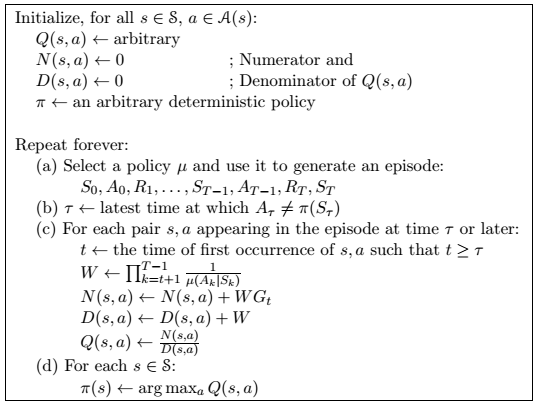
\includegraphics[scale=0.8]{offPolicyPseudo.png}
\caption{Off-Policy Monte Carlo Control Pseudo-code} \label{figure:offPolicy}
\end{figure}


\subsection{\textbf {Sarsa}}
Sarsa is an on-policy method based on model-free action policy estimation. It determines the optimal policy while controlling the MDP with respect to the algorithm which behaves according to the same policy that has been improved.

\subsection*{Sarsa On-Policy TD Control}
Sarsa is an on-policy method of TD learning, whose name (State-Action-Reward-State-Action) is derived from the quintuple $Q(s_t, a_t, r_{t+1}, s_{t+1}, a_{t+1})$, where  $\mathbf{s_t, a_t}$ are the original state and action, $\mathbf{r_{t+1}}$ is the reward observed in the following state and $\mathbf{s_{t+1}, a_{t+1}}$ are the new state-action pair. It expresses the transition from one state-action pair to the next and its update rule is as follow:
\begin{align}
Q(s_t, a_t) \gets Q(s_t, a_t)+\alpha[r_{t+1}+\gamma Q(s_{t+1}, a_{t+1})-Q(s_t, a_t)]
\end{align}\\
The algorithm for Sarsa is presented in Figure 2.3 below:
\begin{figure}[H] \centering
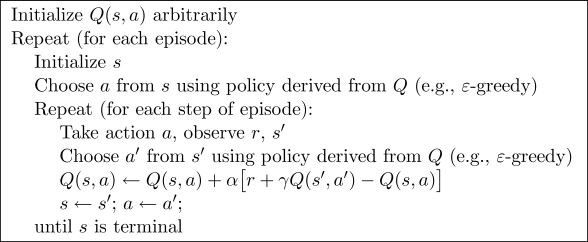
\includegraphics[scale=0.6]{sarsa_algorithm.png}
\caption{Sarsa Pseudo-code} \label{figure:Sarsa}
\end{figure}
As in all on-policy methods, we continually estimate $Q^\pi$ for the behavior policy $\pi$, and at the same time change $\pi$ toward greediness with respect to $Q^\pi$. The update is done after every transition from a nonterminal state $s$. If $s'$ is terminal, then $Q(s',a')$ will be defined as zero. \\


\subsection{\textbf {Q-learning}}
Q-learning is a model-free method which works by learning an action-value function that ultimately gives the expected utility of taking a given action in a given state and following the optimal policy thereafter.  The optimal policy can be constructed by selecting the action with the highest value in each state.
\subsection*{Q-learning Off-policy TD Control}
Q-learning is an off-policy TD control algorithm. It directly approximates the optimal policy $Q^*$ independent from the policy being followed. Its update rule is as follows:
\begin{align}
Q(s_t,a_t) \leftarrow Q(s_t,a_t)+\alpha[r_{t+1}+\gamma \max_a Q(s_{t+1},a)-Q(s_t,a_t)]
\end{align}
The influence of the policy is still in determining which state-action pairs are visited and updated. However, as long as all pairs continue to be updated, which is the minimal requirement to find optimal behavior in the general case, correct convergence shall be reached. Convergence to $Q^*$ with a probability of 1, requires stochastic approximation conditions on the sequence of step-size parameters, i.e. discounted $\epsilon$, $\alpha$. The algorithm is presented in Figure $\ref{figure:Q}$ below:
\begin{figure}[H] \centering
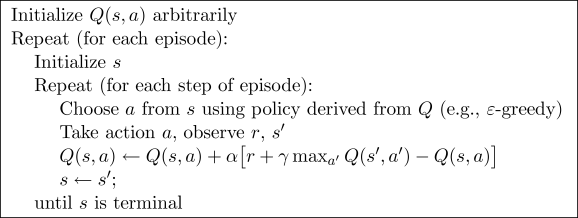
\includegraphics[scale=0.6]{pseudotmp9.png}
\caption{Q-learning: An off-policy TD control algorithm.} \label{figure:Q}
\end{figure}

%\subsection{Reducing the state space}
%\label{reduce}
%Regard the current maximum statespace in the form of 
%\begin{align}
%statespace[predator(x_i,y_j), prey(x_k,y_l)]
%\end{align}
%This statespace has size $11^4$, spanning all possible positions of predator and prey in the $11 \times 11$ grid. Reducing the statespace would mean compressing this table without information loss. Notice the tables of policy and value iteration, table $\ref{pitS}$ and table $\ref{vitS}$, both displaying the values for all possible states by keeping the prey fixed at [5][5]. We can see the same value distribution; and a pattern where the values are proportional to the distance of the predator to the prey. When we look at table $\ref{rVIt}$, where the prey is at [3][2], we notice the exact same value distribution, only translated to the current position of the prey. 

%\indent So a way of reducing the statespace would be by eliminating the representation of the prey within the statespace, by keeping it fixed; we marginalize the conditioning of the prey on the statevalue distribution. We can do this without information loss, by making use of a transform function which translates the actual positions of the prey and predator to an arbitrary one, where the position of the prey has been kept fixed; a statespace where only the position of the predator is variable. In our implementation we make use of one represented by table $\ref{vitS}$.

%\indent The transform function hereby is a simple translation in the following form:
%\begin{align}
%\begin{split}
%P'_{pred} &= \omega((P'_{prey}-P_{prey})+P_{pred}))
%\qquad
%\begin{cases}
%P'_{pred} &= \text{Projected predator position} \\
%P'_{prey} &= \text{Projected prey postion, [5][5] in our case} \\
%P_{prey} &= \text{Actual prey position} \\
%P_{pred} &= \text{Actual predator position}
%\end{cases}
%\end{split}
%\end{align}
%$\omega$ is the wrapper function implemented in our Position class, which takes into consideration that the grid is toroidal. 
%Take table $\ref{rVIt}$ as an aid to illustrate this translation, where we pick position [1][5] as $P_{pred}$ having a certain value (6.440 for the actual state value would not yet be known in the reduced space scenario). [3][2], denotes $P_{prey}$. The value of the state[1][5][3][2] can be looked up by translating this to the calculated reduced space:
%\begin{align}
%\begin{split}
%P'_{pred}
%&=\omega((\begin{bmatrix} 
%5 \\
%5
%\end{bmatrix} -
%\begin{bmatrix}
%3 \\
%2
%\end{bmatrix} )+
%\begin{bmatrix}
%1 \\
%5
%\end{bmatrix}
%\end{split})
%=
%\begin{bmatrix}
%3 \\
%8
%\end{bmatrix}
%\end{align}
%In the calculated reduced space this projected state[3][8][5][5], which has the same relative position of the predator to the prey as in the actual state, conforms with it's value 6.440, the same as we would in a maximum state space scenario. The reduced state space, effectively sized down to $11^2$, results in a lot less memory requirements as well as less computation, which leads us to a faster runtime as seen in table~\ref{runtime}. 

%\begin{table}[H]
%\caption{Runtime of normal and reduced statespace in seconds}
%\centering
 %   \begin{tabular}{|l || l || l |}
 %   \hline
  %  Policy & Normal & Reduced \\ \hline
  %  Policy Evaluation & 13.04 & 0.35\\ \hline
  %  Policy Iteration & 28.27 & 0.28 \\ \hline
  %  Value Iteration & 4.13 & 0.27 \\
  %  \hline
  %  \end{tabular}
  %  \label{runtime}
%\end{table}

%\begin{table}[H]
%\caption{Values from value iteration when the prey is at [3][2]}
%\centering
%\begin{tabular}{l|l*{9}{c}r}
%  \hline
% & 0 & 1 & 2 & 3 & 4 & 5 & 6 & 7 & 8 & 9 & 10 \\ \hline 
%0 & 6.440 & 7.148 & 7.936 & 8.780 & 7.936 & 7.148 & 6.440 & 5.802 & 5.237 & 5.237 & 5.802 \\
%1 & 7.148 & 7.936 & 8.780 & 10.000 & 8.780 & 7.936 & 7.148 & 6.436 & 5.792 & 5.792 & 6.436 \\
%2 & 7.839 & 8.780 & 10.000 & 0.000 & 10.000 & 8.780 & 7.839 & 6.997 & 6.251 & 6.251 & 6.997 \\
%3 & 7.148 & 7.936 & 8.780 & 10.000 & 8.780 & 7.936 & 7.148 & 6.436 & 5.792 & 5.792 & 6.436 \\
%4 & 6.440 & 7.148 & 7.936 & 8.780 & 7.936 & 7.148 & 6.440 & 5.802 & 5.237 & 5.237 & 5.802 \\
%5 & 5.802 & 6.440 & 7.148 & 7.839 & 7.148 & 6.440 & 5.802 & 5.228 & 4.742 & 4.742 & 5.228 \\
%6 & 5.228 & 5.802 & 6.436 & 6.997 & 6.436 & 5.802 & 5.228 & 4.712 & 4.291 & 4.291 & 4.712 \\
%7 & 4.742 & 5.237 & 5.792 & 6.251 & 5.792 & 5.237 & 4.742 & 4.291 & 3.883 & 3.883 & 4.291 \\
%8 & 4.742 & 5.237 & 5.792 & 6.251 & 5.792 & 5.237 & 4.742 & 4.291 & 3.883 & 3.883 & 4.291 \\
%9 & 5.228 & 5.802 & 6.436 & 6.997 & 6.436 & 5.802 & 5.228 & 4.712 & 4.291 & 4.291 & 4.712 \\
%10&5.802 & 6.440 & 7.148 & 7.839 & 7.148 & 6.440 & 5.802 & 5.228 & 4.742 & 4.742 & 5.228
%\end{tabular}
%\label{rVIt}
%\end{table}
%\label{trans}

\section{Experiments and Results}
\label{results}

\subsection{Theoretical Differences}
The differences that appear while considering the off-policy Monte Carlo and on-policy Monte Carlo methods are related to the theoretical contrast between an off-policy and an on-policy. In the on-policy method, the agent commits to always exploring and tries to find the best policy that still explores. In off-policy method, the agent also explores, but learns a deterministic optimal policy that may be unrelated to the policy followed. If the on-policy  method is generally soft (e.g. $\epsilon$-soft policy) and improves the policy that is used to make decision, then the off-policy method is composed of two separated functions (behavior policy and target policy) which can be considered an advantage, because the target policy may be deterministic (e.g. greedy), while the behavior policy can continue to sample all possible actions. \\
The same differentiation can be applied between Sarsa and Q-learning. Sarsa is useful when you want to optimize a bounded exploratory policy of an agent while exploring - it is on-policy. When it's possible to separate the policies, meaning the policy being learned could be unrelated to the one followed, it might be more advantageous to use Q-learning, which is an off-policy method. Difference between TD and MC methods are that the aforementioned bootstrap; they update estimates based on other learned estimates, without waiting for a final outcome like MC.

\subsection{Q-learning with $\epsilon$-greedy: experiments on $\alpha$ and $\gamma$}
\subsubsection*{Q-learning with $\epsilon$-greedy: experiments on $\alpha$}
Recall the update rule for Q-learning:
\begin{align}
Q(s_t,a_t) \leftarrow Q(s_t,a_t)+\alpha[r_{t+1}+\gamma \max_a Q(s_{t+1},a)-Q(s_t,a_t)]
\end{align}
We see that both $\alpha$ and $\gamma$ influence the rate of update ("learning-rate") on the current $Q$ value of a state action pair. While $\alpha$ is overall inclusive and taking the observed next reward into account, $\gamma$ controls solely the ratio between the current $Q$ value and that of the next state. Taking this into account we will expect to have a slower convergent rate for low values of $\alpha$ and $\gamma$. The question remains how much they will influence the convergence to the optimal policy in the long run.

We experiment with the following values for $\alpha$: 0.1, 0.2, 0.3, 0.4 and 0.5, with the following conditions on the experimental setup:
\begin{table}[H]
\caption{Experimental setup for testing $\alpha$}
\centering
\begin{tabular}{|l|r|}
\hline
Parameters & Value \\\hline
$\epsilon$ & 0.1 \\\hline
initial Q & 15 \\\hline
$\gamma$ & 0.9\\\hline
$N$ runs & 20000\\\hline
\end{tabular}
\label{expSetupAlpha}
\end{table}
The results from the experiments are displayed below. In order to give a comprehensible graph, we plot the average of batches of a 100 over the 20000. We see that lower values of $\alpha$ give slower convergence as expected, which is clearly  illustrated in Figure \ref{figure:alphafirst20} and all of the values converge to average sub 10 capture times after about 1250 runs. Less clear is its influence in the long run, as displayed in Figure \ref{figure:alphalast20}. Capture times are fluctuating between values of 5 and 6, seemingly giving equal performance rates for all values of $\alpha$ in the long run.
%\begin{table}[H]
%\caption{Convergence for different values of $\alpha$}
%\centering
%\begin{tabular} {cc}
%  \num\putindeepbox[7pt]{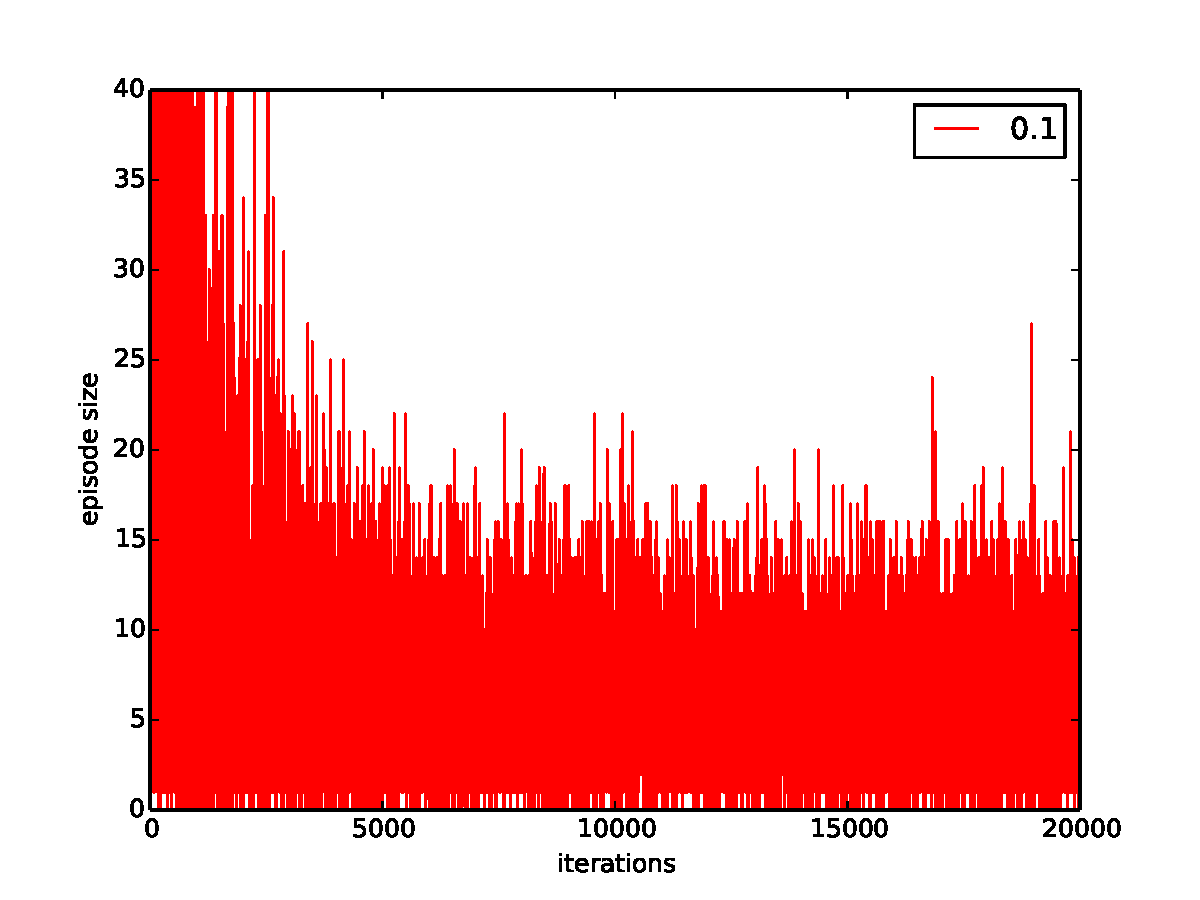
\includegraphics[scale=0.3]{alpha0_1.pdf}}
%    & \num\putindeepbox[7pt]{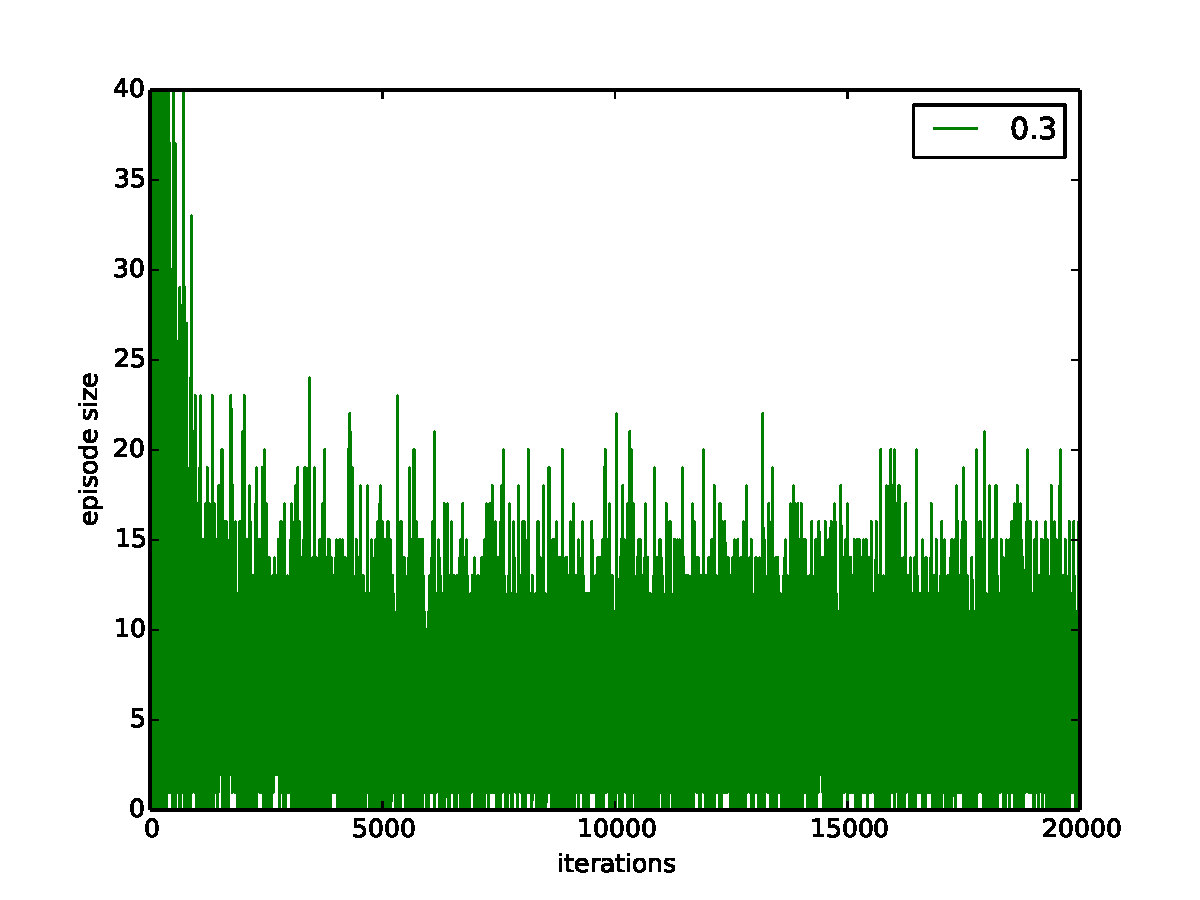
\includegraphics[scale=0.3]{alpha0_3.pdf}} \\
%  \num\putindeepbox[7pt]{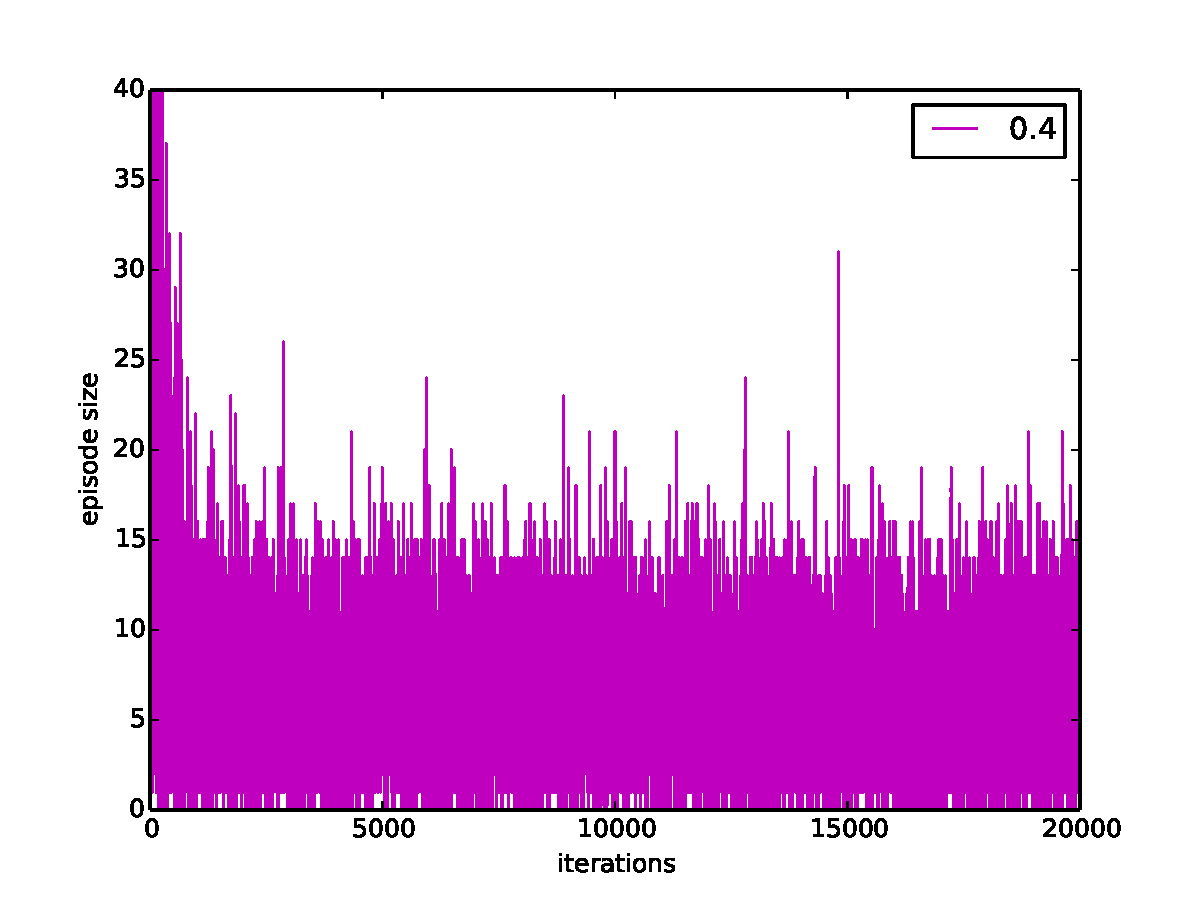
\includegraphics[scale=0.3]{alpha0_4.pdf}}
%    & \num\putindeepbox[7pt]{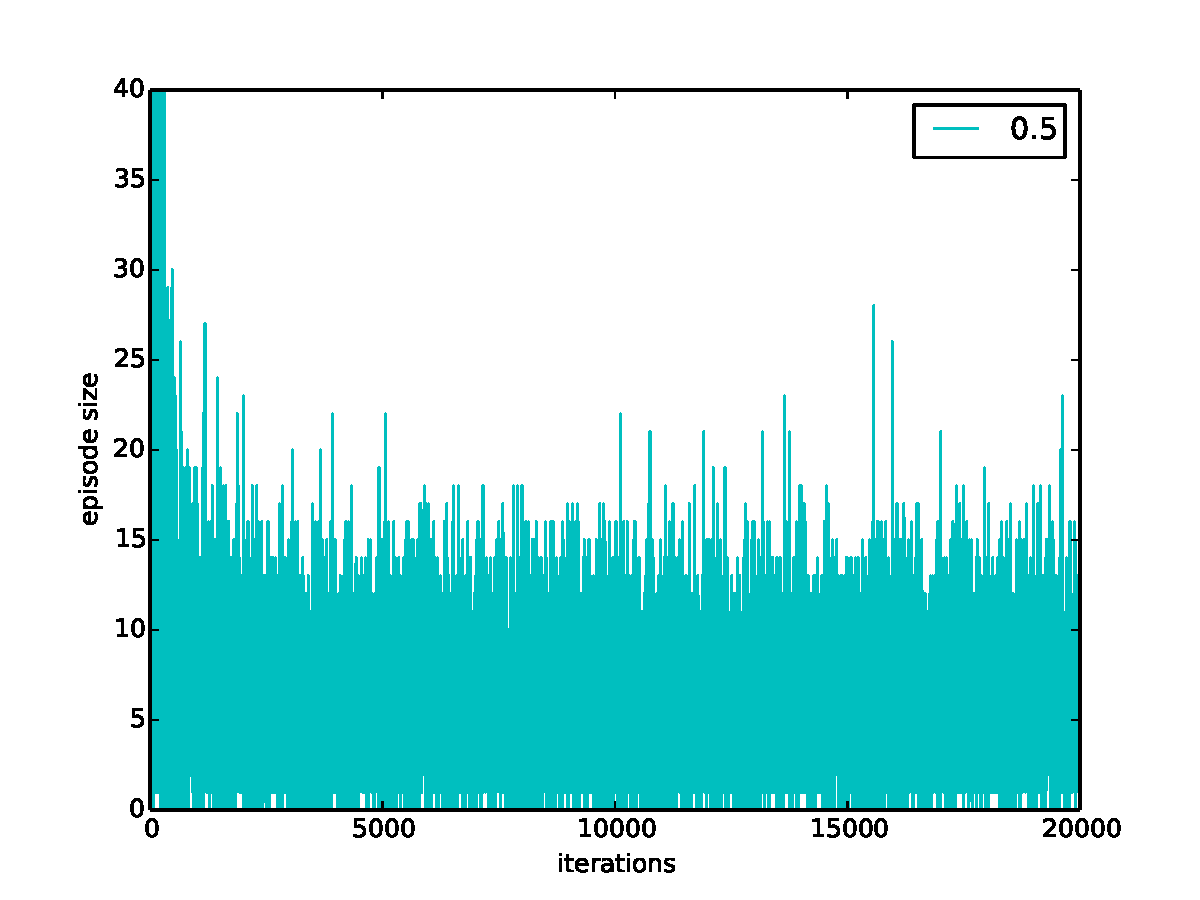
\includegraphics[scale=0.3]{alpha0_5.pdf}} \\
%\end{tabular}
%\label{table:qalpha}
%\end{table}
%
\begin{figure}[H] \centering
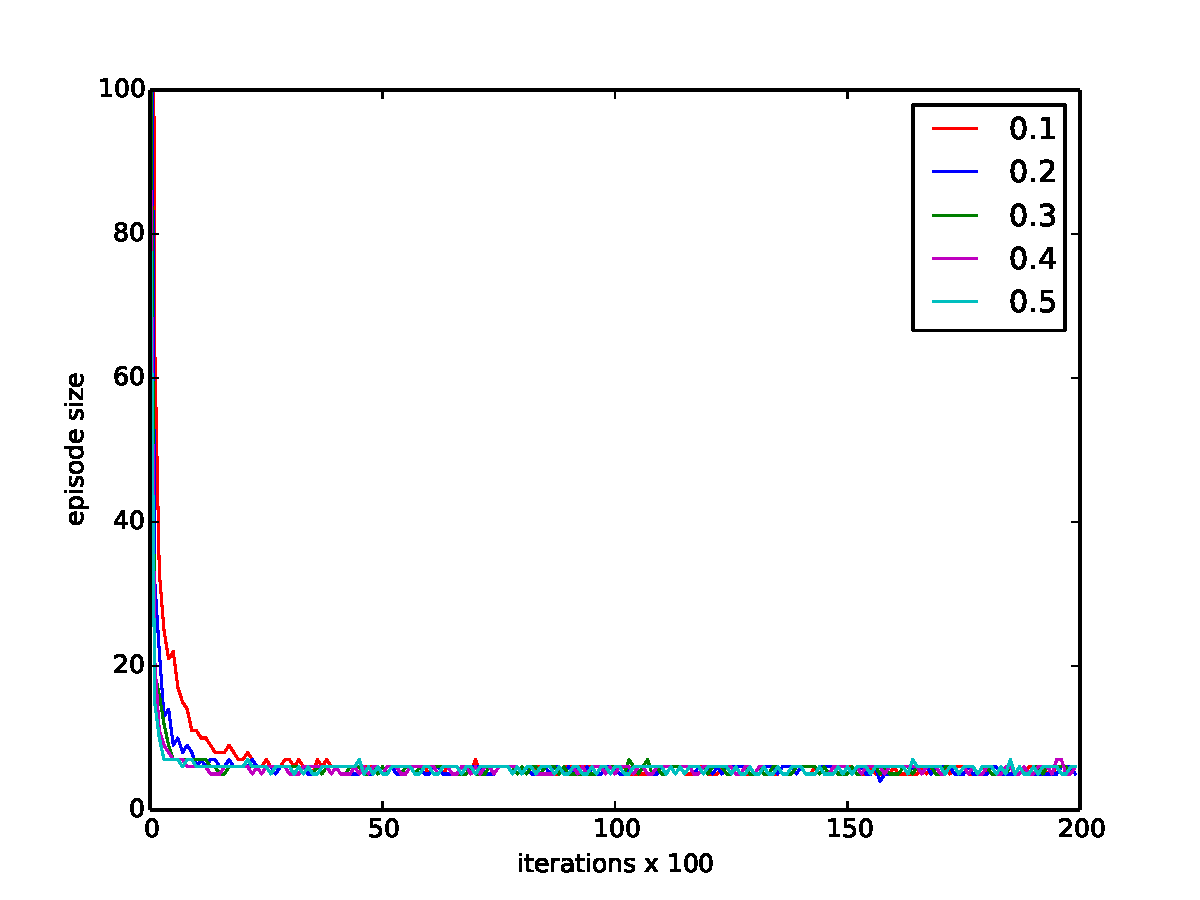
\includegraphics[scale=0.5]{alphaOverview.pdf}
\caption{Convergence overview for different values of $\alpha$.} 
\label{figure:alphaOverview}
\end{figure}
\begin{figure}[H] \centering
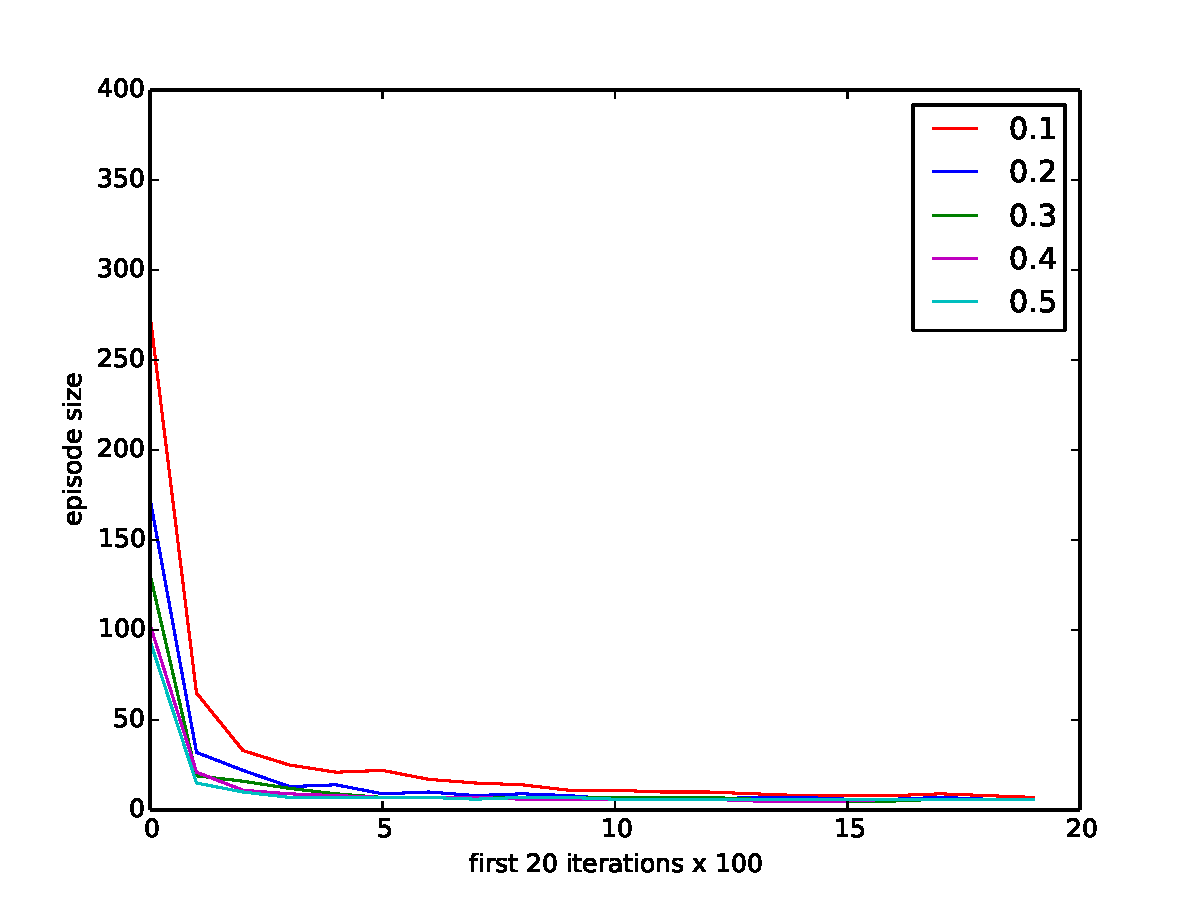
\includegraphics[scale=0.5]{alphafirst20x100.pdf}
\caption{Convergence for different values of $\alpha$ in the initial 2000 runs.} 
\label{figure:alphafirst20}
\end{figure}
\begin{figure}[H] \centering
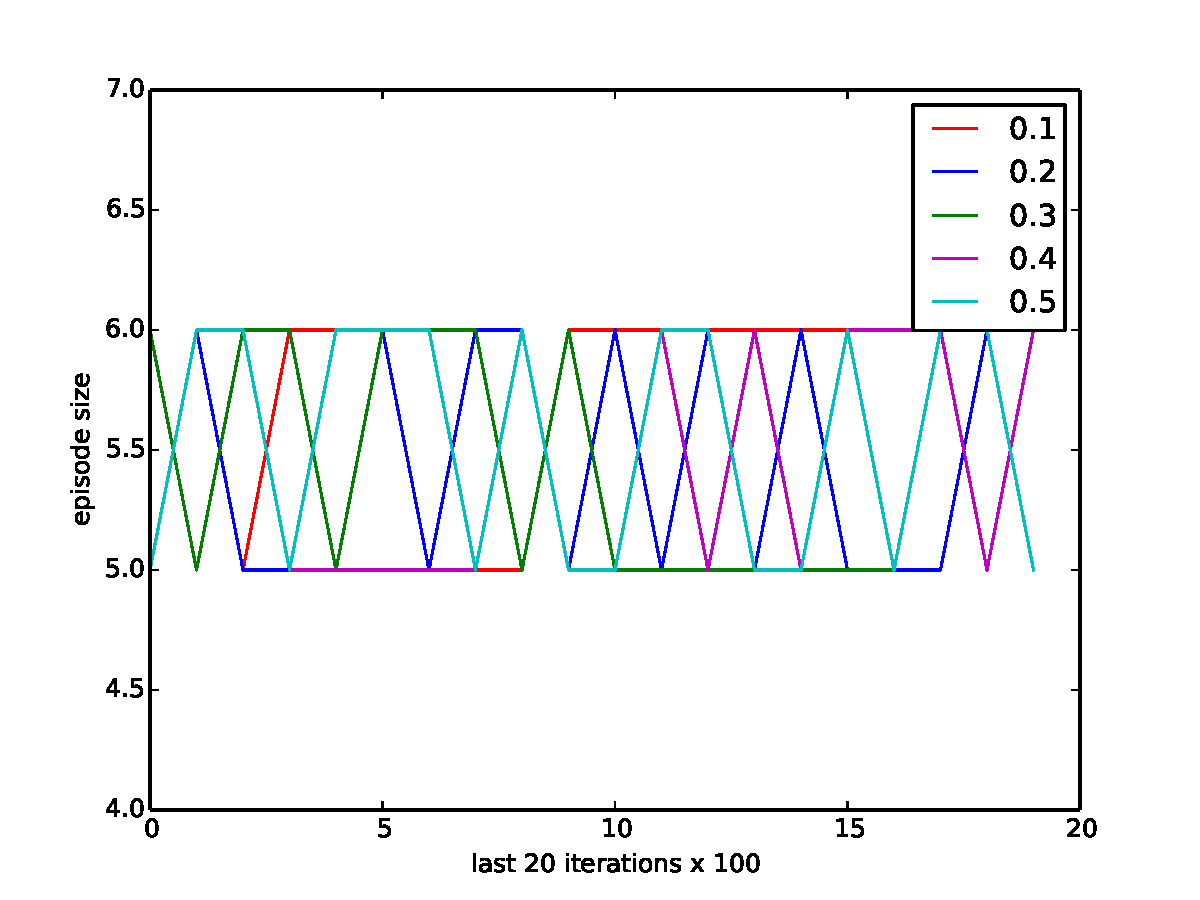
\includegraphics[scale=0.5]{alphalast20x100.pdf}
\caption{Convergence for different values of $\alpha$ in the last 2000 runs.} 
\label{figure:alphalast20}
\end{figure}
Since we acquired the optimal policy from value iteration in the first assignment, displayed in Table \ref{table:optimalPolicy}, we could plot the performance in terms of a ratio from the optimal policy. We take the argmax of the Q-table after a test run and compare that to the aforementioned optimal policy. Its ratio will define its optimality:
\begin{align}
Optimality = \frac{Diff(\text{nr of optimal actions})}{Total(\text{number of actions from the optimal policy})}
\end{align}

\begin{table}[H]
\caption{Optimal policy in the reduced state space from Value Iteration given the prey at (5,5).}
\centering
\begin{tabular}{l|l*{9}{c}r}
  \hline
 & 0 & 1 & 2 & 3 & 4 & 5 & 6 & 7 & 8 & 9 & 10 \\ \hline
0 & $\downarrow$& $\rightarrow$& $\rightarrow$& $\rightarrow$& $\downarrow$& $\downarrow$& $\downarrow$& $\leftarrow$& $\leftarrow$& $\leftarrow$& $\downarrow$ \\
1 & $\downarrow$& $\downarrow$& $\rightarrow$& $\downarrow$& $\downarrow$& $\downarrow$& $\downarrow$& $\downarrow$& $\leftarrow$& $\downarrow$& $\downarrow$ \\
2 & $\downarrow$& $\downarrow$& $\downarrow$& $\downarrow$& $\downarrow$& $\downarrow$& $\downarrow$& $\downarrow$& $\downarrow$& $\downarrow$& $\downarrow$ \\
3 & $\downarrow$& $\rightarrow$& $\rightarrow$& $\downarrow$& $\downarrow$& $\downarrow$& $\downarrow$& $\downarrow$& $\leftarrow$& $\leftarrow$& $\downarrow$ \\
4 & $\rightarrow$& $\rightarrow$& $\rightarrow$& $\rightarrow$& $\downarrow$& $\downarrow$& $\downarrow$& $\leftarrow$& $\leftarrow$& $\leftarrow$& $\leftarrow$ \\
5 & $\rightarrow$& $\rightarrow$& $\rightarrow$& $\rightarrow$& $\rightarrow$& P& $\leftarrow$& $\leftarrow$& $\leftarrow$& $\leftarrow$& $\leftarrow$ \\
6 & $\rightarrow$& $\rightarrow$& $\rightarrow$& $\rightarrow$& $\uparrow$& $\uparrow$& $\uparrow$& $\leftarrow$& $\leftarrow$& $\leftarrow$& $\leftarrow$ \\
7 & $\uparrow$& $\rightarrow$& $\rightarrow$& $\uparrow$& $\uparrow$& $\uparrow$& $\uparrow$& $\uparrow$& $\leftarrow$& $\leftarrow$& $\uparrow$ \\
8 & $\uparrow$& $\uparrow$& $\uparrow$& $\uparrow$& $\uparrow$& $\uparrow$& $\uparrow$& $\uparrow$& $\uparrow$& $\uparrow$& $\uparrow$ \\
9 & $\uparrow$& $\uparrow$& $\rightarrow$& $\uparrow$& $\uparrow$& $\uparrow$& $\uparrow$& $\uparrow$& $\leftarrow$& $\uparrow$& $\uparrow$ \\
10 & $\uparrow$& $\rightarrow$& $\rightarrow$& $\rightarrow$& $\uparrow$& $\uparrow$& $\uparrow$& $\leftarrow$& $\leftarrow$& $\leftarrow$& $\uparrow$ \\
\end{tabular}
\label{table:optimalPolicy}
\end{table}

The results, plotted as the average of batches of a 100 over the 20000, are displayed in Figure \ref{figure:alphaOpti}. For the initial stage of the runs we see that convergence confirm that what was expected and earlier graphed in the average capture times. Far more interesting is the performance in the long run for different values of $\alpha$. By comparing directly in the optimal policy space we essentially reduce the noise from the output of the many runs, and thereby reducing the effect of the random element of the prey and the initial start conditions within each run. Since the latter could randomly favor a run, and thereby it's capture time, regardless of the policy following. 

In a state space this small, all policies would converge to similar capture times in the end, caused by the stochastic elements in which each run is initiated. Looking directly at the optimality graph however, we can say that, although its initial convergence is slower, an $\alpha$ value of 0.2 actually performs better in the end. Further tests below would present us, whether this claim withholds or there might be more interesting interactions between the parameters tested.
\begin{figure}[H] \centering
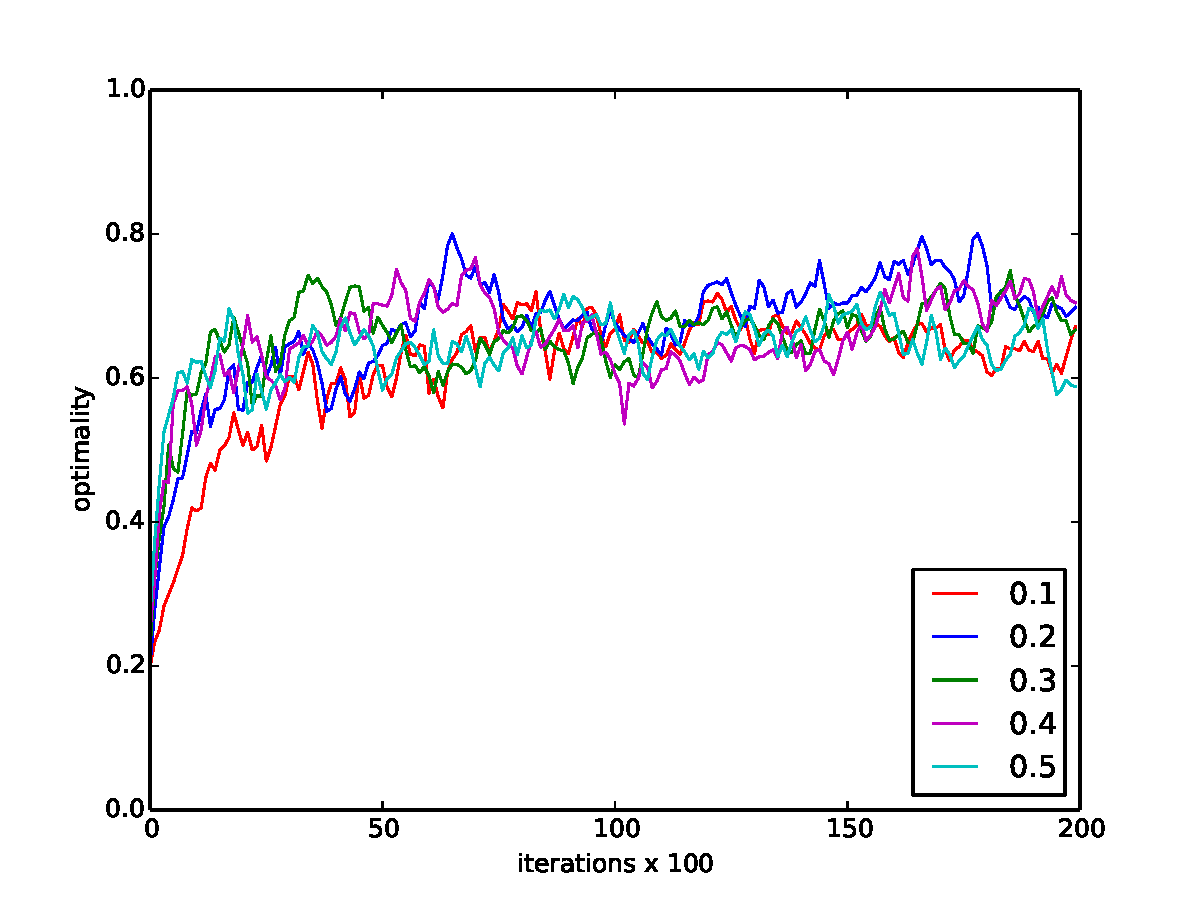
\includegraphics[scale=0.6]{alphaOptimality.pdf}
\caption{Optimality for different values of $\alpha$ as a ratio to the optimal policy.} 
\label{figure:alphaOpti}
\end{figure}
\subsubsection*{Q-learning with $\epsilon$-greedy: experiments on $\gamma$}
Initial tests with $\gamma$ are done with the following values: 0.1, 0.2, 0.5, 0.7 and 0.9, and with the following conditions on the experimental setup:
\begin{table}[H]
\caption{Experimental setup for testing $\gamma$}
\centering
\begin{tabular}{|l|r|}
\hline
Parameters & Value \\\hline
$\epsilon$ & 0.1 \\\hline
initial Q & 15 \\\hline
$\alpha$ & 0.2\\\hline
$N$ runs & 20000\\\hline
\end{tabular}
\label{expSetupGamma}
\end{table}
Again, the results are plotted with the average of batches of a 100 over the 20000, which can be assumed for all of the future experiments, unless stated otherwise. The outcome is comparable to that of $\alpha$; lower values of $\gamma$ give slower convergence as expected, which is clearly illustrated in Figure \ref{figure:gammafirst20}. Interesting is the out-lier start of $\gamma$ value 0.9, see Figure \ref{figure:gammafirst20}. This might be caused by unfavorable stochastic conditions or too greedy initial faulty learning. However, it quickly adapts and makes a sharp dive, overtaking the other values after 200 runs.

All of the values converge to average sub 10 capture times after about 1250 runs, saying very little of the optimality of the policy being learned in the long run. Capture times are eventually bouncing between values of 5 and 6, apart of an out-lier value of 7 for $\gamma$ value 0.7, which might be due to effects as earlier described, see Figure \ref{figure:gammalast20}.
\begin{figure}[H] \centering
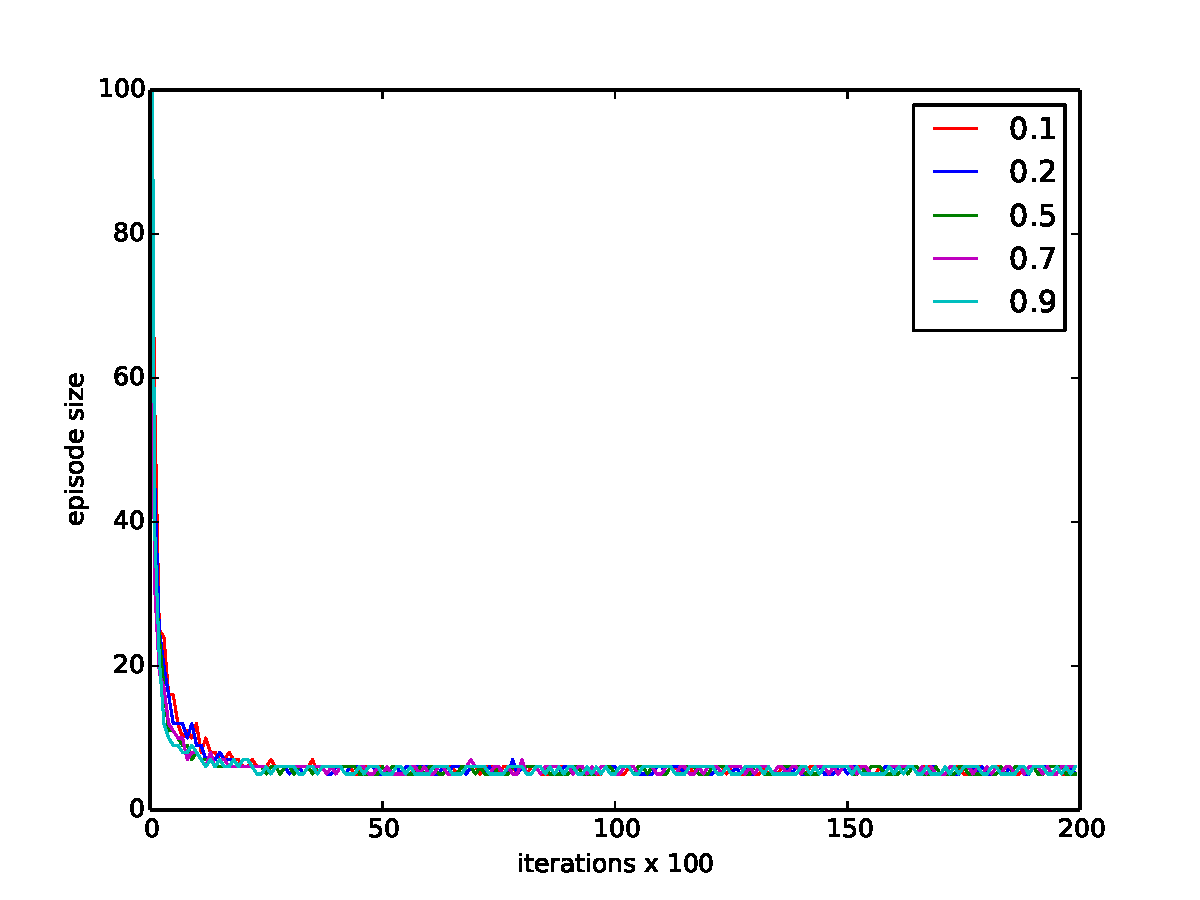
\includegraphics[scale=0.5]{gammaOverview.pdf}
\caption{Convergence overview for different values of $\gamma$.} 
\label{figure:gammaOverview}
\end{figure}
\begin{figure}[H] \centering
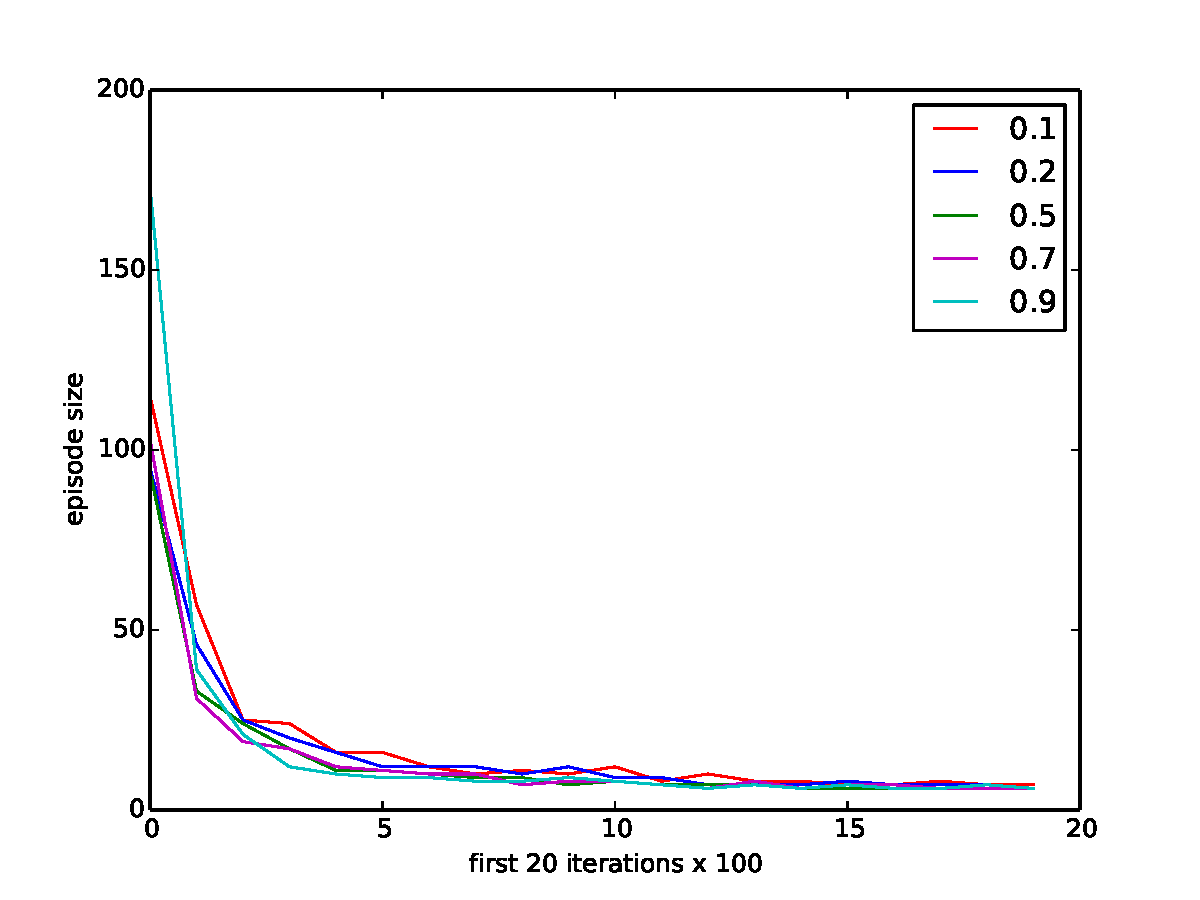
\includegraphics[scale=0.5]{gammafirst20x100.pdf}
\caption{Convergence for different values of $\gamma$ in the initial 2000 runs.} 
\label{figure:gammafirst20}
\end{figure}
\begin{figure}[H] \centering
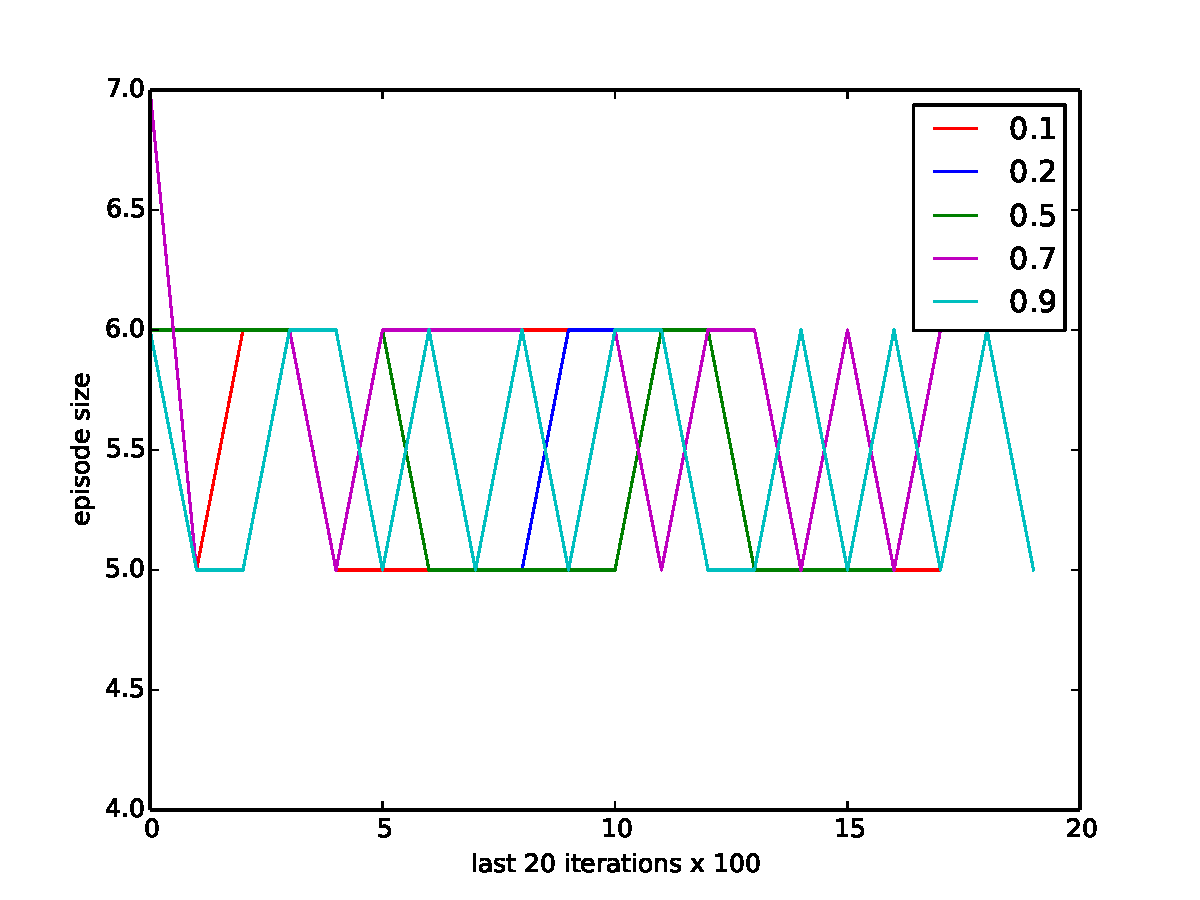
\includegraphics[scale=0.5]{gammalast20x100.pdf}
\caption{Convergence for different values of $\gamma$ in the last 2000 runs.} 
\label{figure:gammalast20}
\end{figure}
If we look directly into policy optimality space, we see that lower values of $\gamma$ show promising results in the end. Interesting is the climb of $\gamma$ value 0.9 therein. This might be due to negating effects to the chosen lower value of $\alpha$ of 0.2. Runs with the contrasting value of 0.5 for $\alpha$ are plotted against these promising values of $\gamma$ to see if this is indeed the case, see Figure \ref{figure:alphagammaOpti}.
\begin{figure}[H] \centering
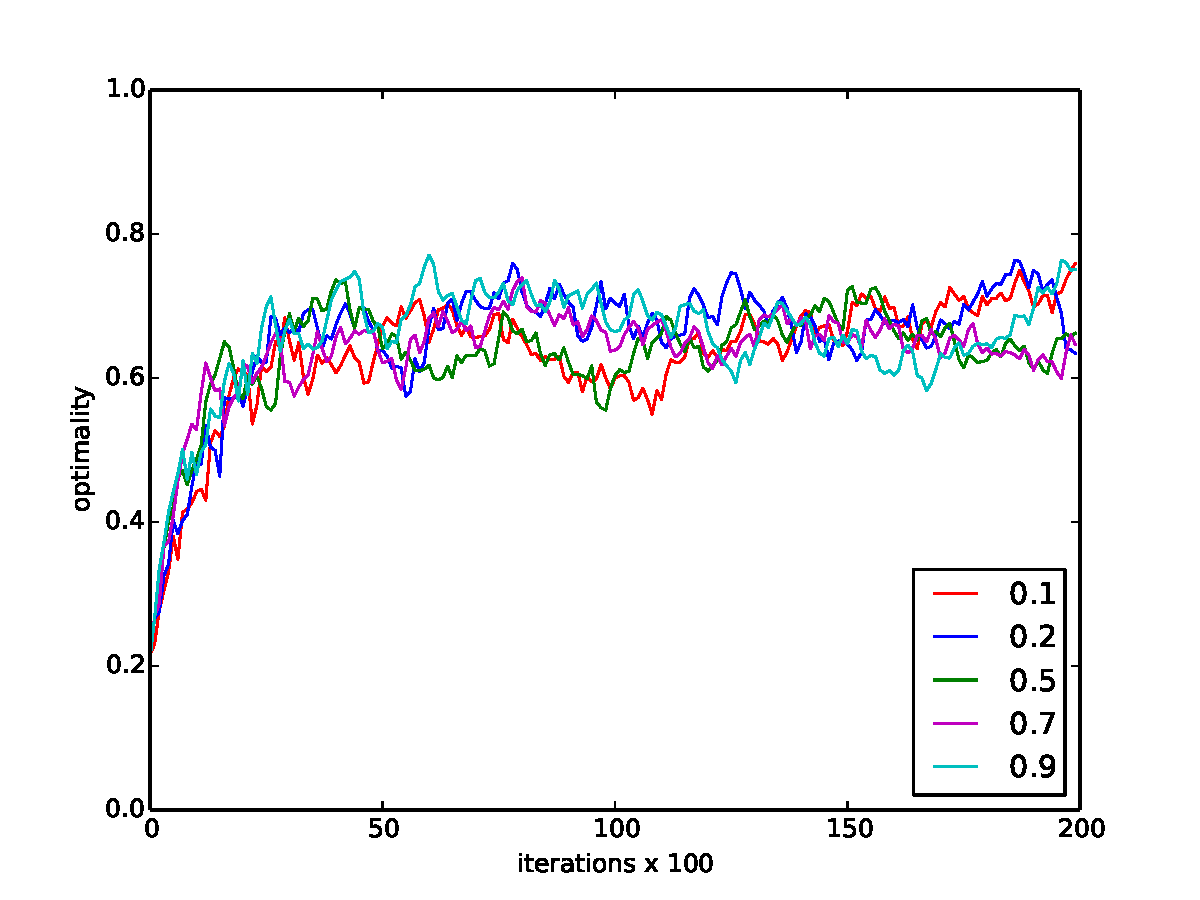
\includegraphics[scale=0.5]{gammaOptimality.pdf}
\caption{Optimality for different values of $\gamma$ as a ratio to the optimal policy.} 
\label{figure:gammaOpti}
\end{figure}
\begin{figure}[H] \centering
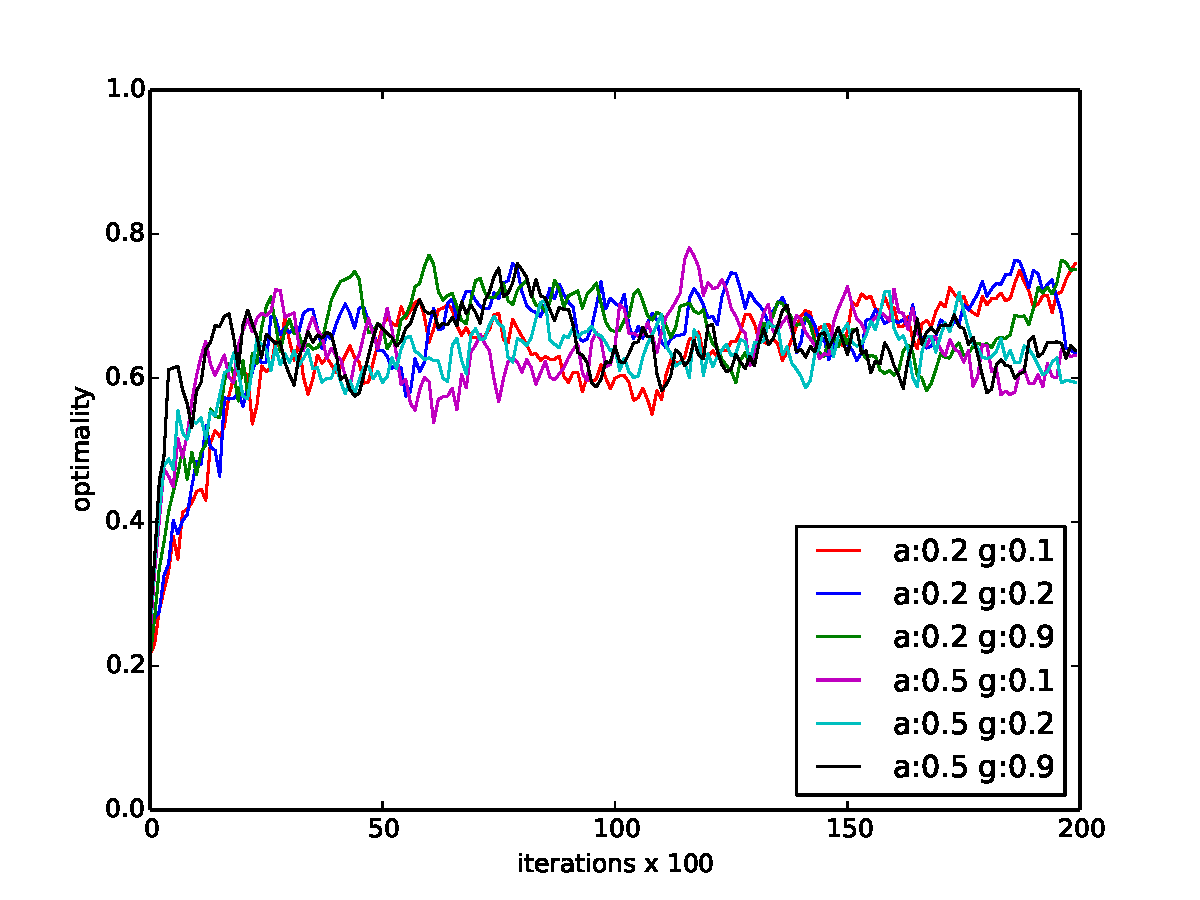
\includegraphics[scale=0.5]{alphaGammaOptimality.pdf}
\caption{Optimality with the interaction of $\alpha$ and $\gamma$.} 
\label{figure:alphagammaOpti}
\end{figure}
Indeed, higher values of $\alpha$ have a much greater impact as earlier foretold (overall inclusive influence on the update). We see a fast initial climb, but in the long run will impair further convergence and the negating effect of a lower $\gamma$ has little influence.

\subsection{Q-learning with $\epsilon$-greedy: experiments on $\epsilon$ and optimistic initialization}
\subsubsection*{Q-learning with $\epsilon$-greedy: experiments on $\epsilon$}
We experiment with the following values for $\epsilon$: 0.001, 0.1, 0.2, 0.3, and 0.5, with the following conditions on the experimental setup:
\begin{table}[H]
\caption{Experimental setup for testing $\epsilon$}
\centering
\begin{tabular}{|l|r|}
\hline
Parameters & Value \\\hline
$\alpha$ & 0.2 \\\hline
initial Q & 15 \\\hline
$\gamma$ & 0.1\\\hline
$N$ runs & 20000\\\hline
\end{tabular}
\label{expSetupEpsilon}
\end{table}
$\epsilon$ in $\epsilon$-greedy controls the probability in which a random action is selected. Lower values of $\epsilon$ will steer its policy to a greedy action selection, while higher values will favor exploration more, thus a faster initial  convergence, yet a less optimal policy in the end. With the earlier chosen values of $\epsilon$ we try to reflect that in our graphs. From the results below, we see that high values of $\epsilon$ show fast initial convergence due to exploration, but give a slow convergence rate in the second stage. They even converge to a less optimal policy in the end. The average capture times are higher overall and its policy is highly fluctuating, as can be seen in Figure \ref{figure:epsilonOpti}. Without discount of $\epsilon$ in the long run the algorithm is always stuck in exploration mode due to the fixed degree of $\epsilon$.

On the other hand the relatively extreme low value of 0.001 for $\epsilon$ causes the algorithm to slowly climb and stabilize much more in the long run, giving it the best final average capture time, even though it is not peaking in the ratio of its optimality. The low value gives the algorithm its robustness in the end, not "being tempted" by exploration.
\begin{figure}[H] \centering
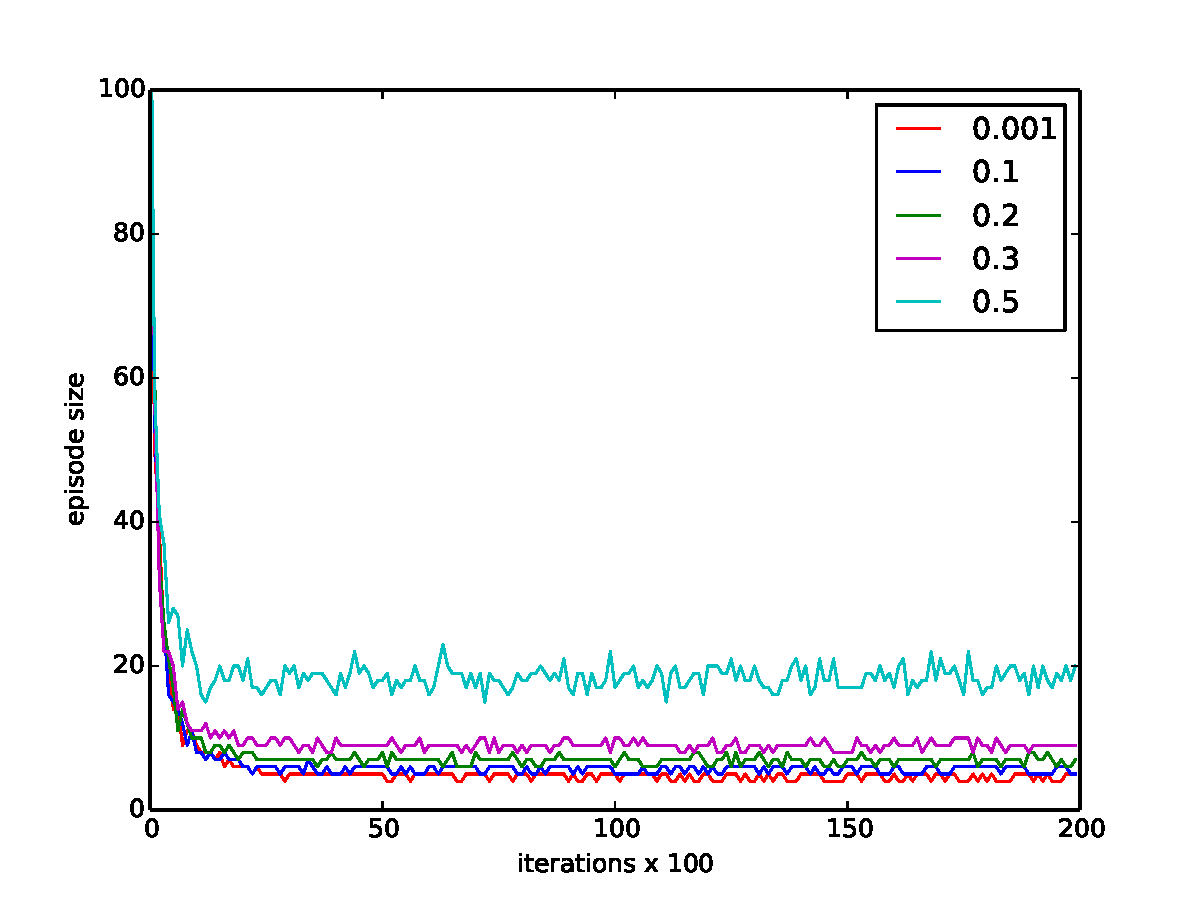
\includegraphics[scale=0.5]{epsilonOverview.pdf}
\caption{Convergence overview for different values of $\epsilon$.} 
\label{figure:epsilonOverview}
\end{figure}
\begin{figure}[H] \centering
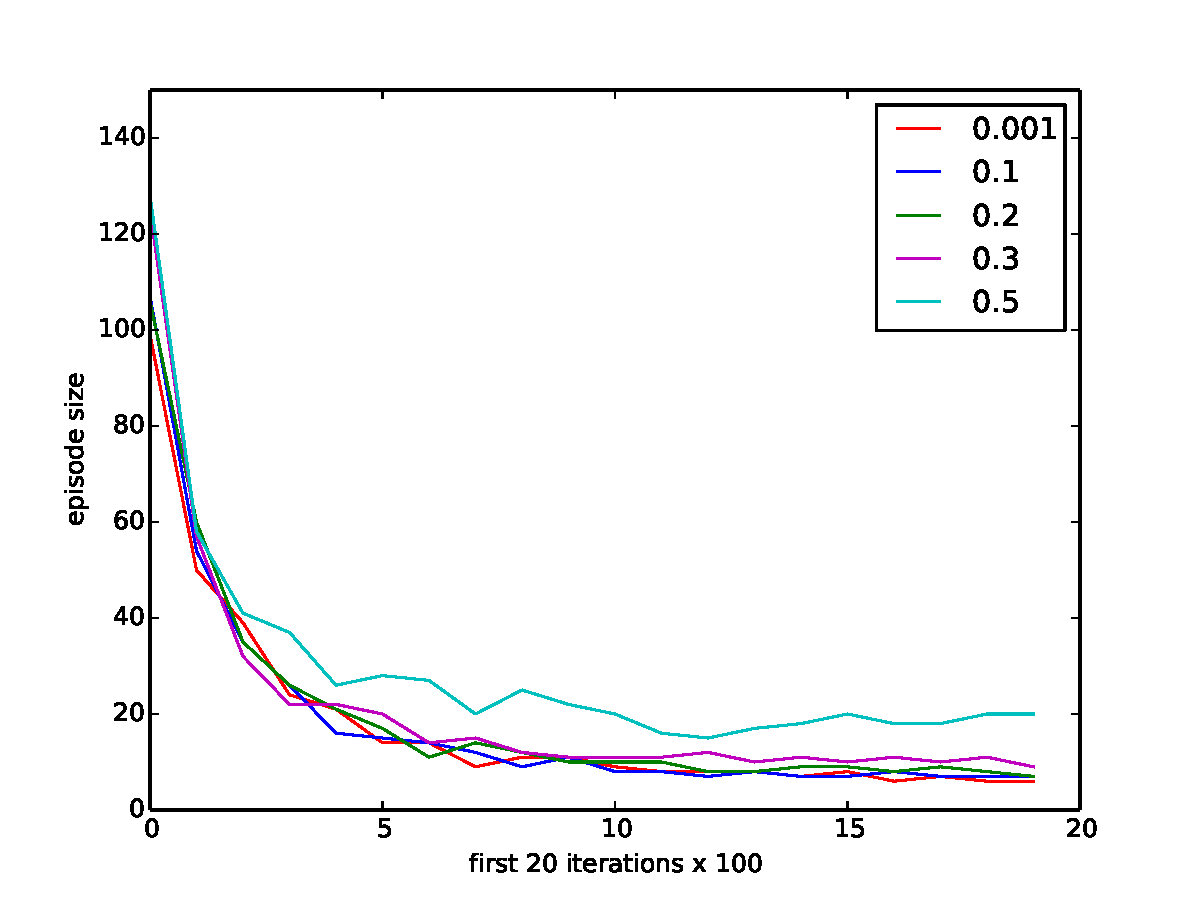
\includegraphics[scale=0.5]{epsilonfirst20x100.pdf}
\caption{Convergence for different values of $\epsilon$ in the initial 2000 runs.} 
\label{figure:epsilonfirst20}
\end{figure}
\begin{figure}[H] \centering
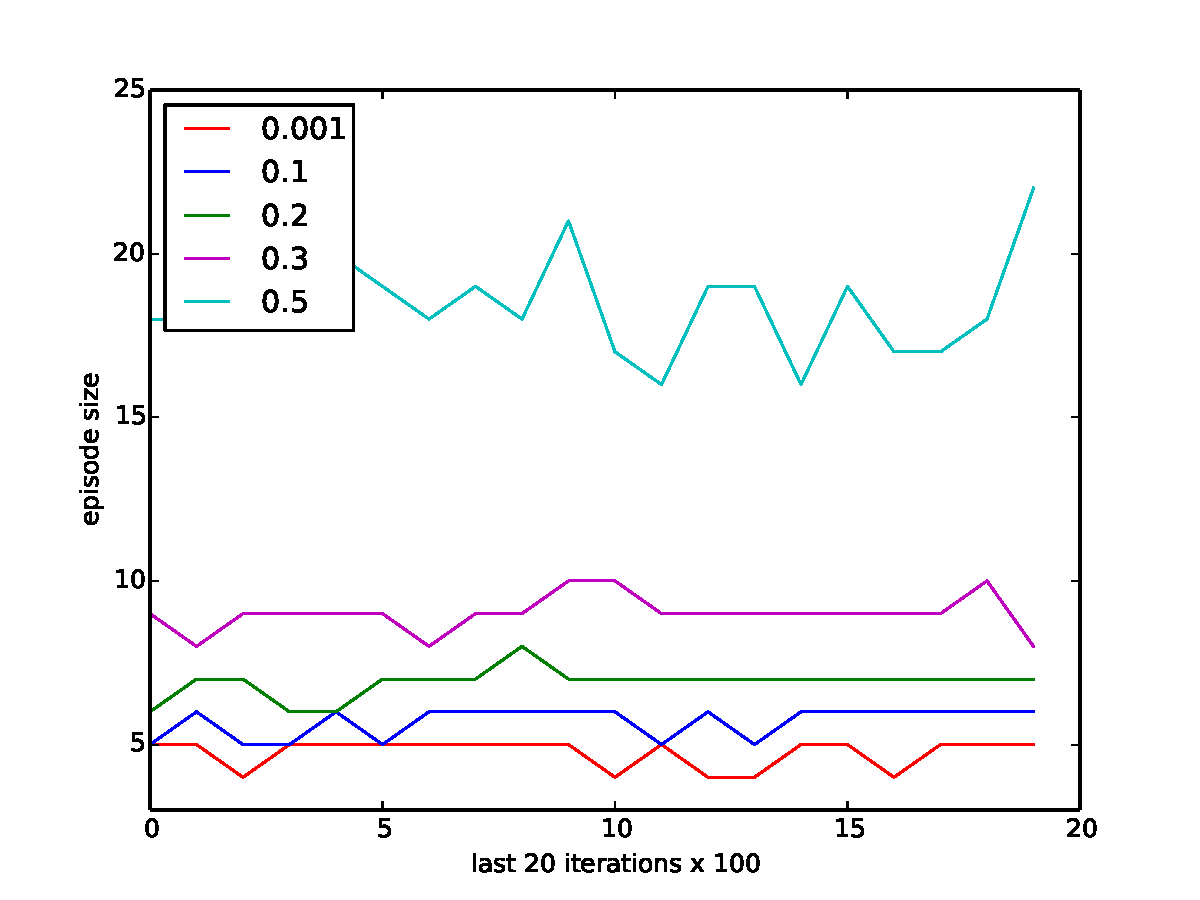
\includegraphics[scale=0.5]{epsilonlast20x100.pdf}
\caption{Convergence for different values of $\epsilon$ in the last 2000 runs.} 
\label{figure:epsilonlast20}
\end{figure}
\begin{figure}[H] \centering
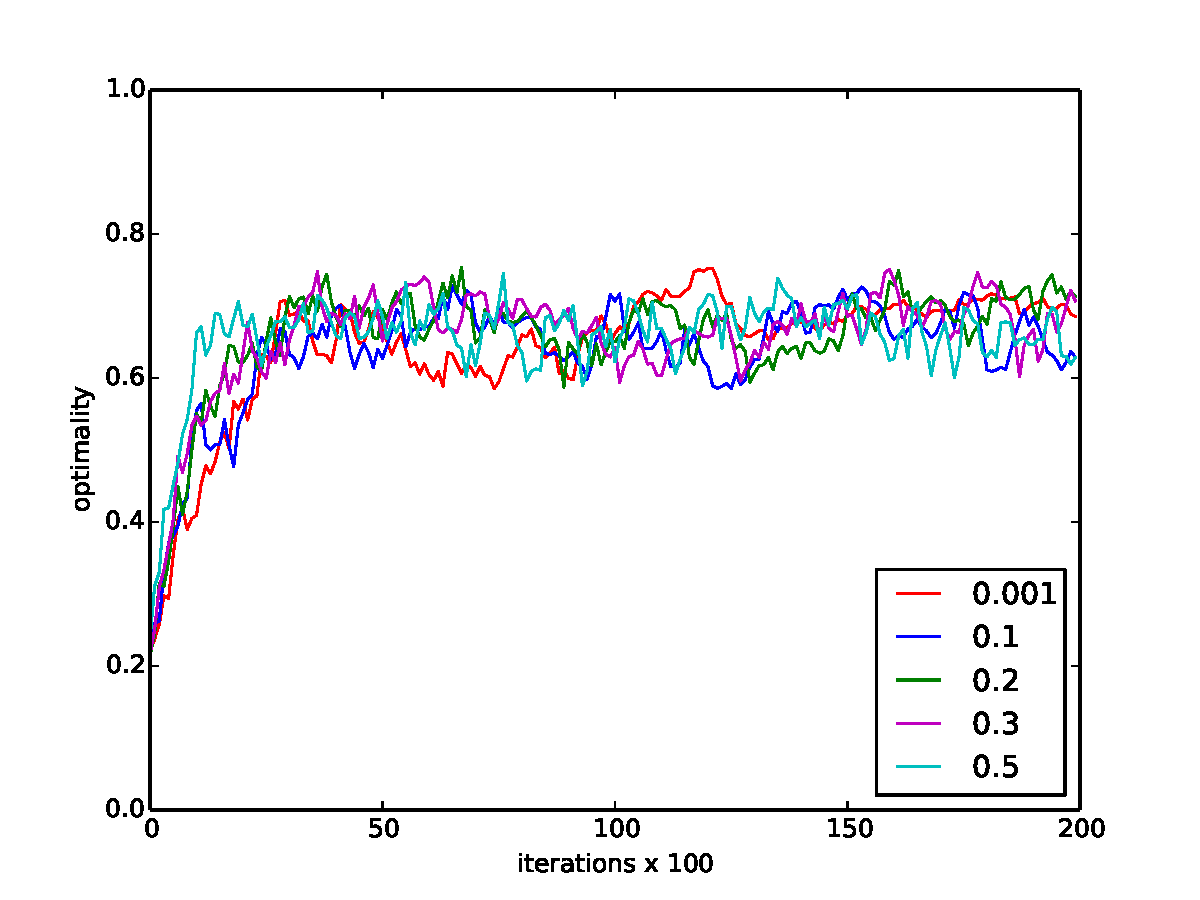
\includegraphics[scale=0.6]{epsilonOptimality.pdf}
\caption{Optimality for different values of $\epsilon$ as a ratio to the optimal policy} 
\label{figure:epsilonOpti}
\end{figure}
\subsubsection*{Q-learning with $\epsilon$-greedy: experiments on optimistic initialization}
For the optimistic initialization of the Q-table we decided to start with the values derived from the optimal policy acquired from Value Iteration, see Table \ref{table:vi}. Actions corresponding to those of the optimal policy, see Table \ref{table:optimalPolicy}, will get its assigned value, while others are given the value 0. Further tests are done with initialization values of 0, 5 and 10, added to the value of 15 of earlier experiments. Conditions on the experimental setup are as follow:
\begin{table}[H]
\caption{Experimental setup for testing optimistic initialization}
\centering
\begin{tabular}{|l|r|}
\hline
Parameters & Value \\\hline
$\alpha$ & 0.2 \\\hline
$\epsilon$ & 0.1 \\\hline
$\gamma$ & 0.1\\\hline
$N$ runs & 20000\\\hline
\end{tabular}
\label{expSetupOptimInit}
\end{table}
\begin{table}[H]
\caption{Values from value iteration when the prey is at [5][5]}
\centering
\begin{tabular}{l|l*{9}{c}r}
  \hline
 & 0 & 1 & 2 & 3 & 4 & 5 & 6 & 7 & 8 & 9 & 10 \\ \hline 
0 & 3.883 & 4.291 & 4.742 & 5.237 & 5.792 & 6.251 & 5.792 & 5.237 & 4.742 & 4.291 & 3.883 \\
1 & 4.291 & 4.712 & 5.228 & 5.802 & 6.436 & 6.997 & 6.436 & 5.802 & 5.228 & 4.712 & 4.291 \\
2 & 4.742 & 5.228 & 5.802 & 6.440 & 7.148 & 7.839 & 7.148 & 6.440 & 5.802 & 5.228 & 4.742 \\
3 & 5.237 & 5.802 & 6.440 & 7.148 & 7.936 & 8.780 & 7.936 & 7.148 & 6.440 & 5.802 & 5.237 \\
4 & 5.792 & 6.436 & 7.148 & 7.936 & 8.780 & 10.000 & 8.780 & 7.936 & 7.148 & 6.436 & 5.792 \\
5 & 6.251 & 6.997 & 7.839 & 8.780 & 10.000 & 0.000 & 10.000 & 8.780 & 7.839 & 6.997 & 6.251 \\
6 & 5.792 & 6.436 & 7.148 & 7.936 & 8.780 & 10.000 & 8.780 & 7.936 & 7.148 & 6.436 & 5.792 \\
7 & 5.237 & 5.802 & 6.440 & 7.148 & 7.936 & 8.780 & 7.936 & 7.148 & 6.440 & 5.802 & 5.237 \\
8 & 4.742 & 5.228 & 5.802 & 6.440 & 7.148 & 7.839 & 7.148 & 6.440 & 5.802 & 5.228 & 4.742 \\
9& 4.291 & 4.712 & 5.228 & 5.802 & 6.436 & 6.997 & 6.436 & 5.802 & 5.228 & 4.712 & 4.291 \\
10& 3.883 & 4.291 & 4.742 & 5.237 & 5.792 & 6.251 & 5.792 & 5.237 & 4.742 & 4.291 & 3.883
\end{tabular}
\label{table:vi}
\end{table}
\begin{figure}[H] \centering
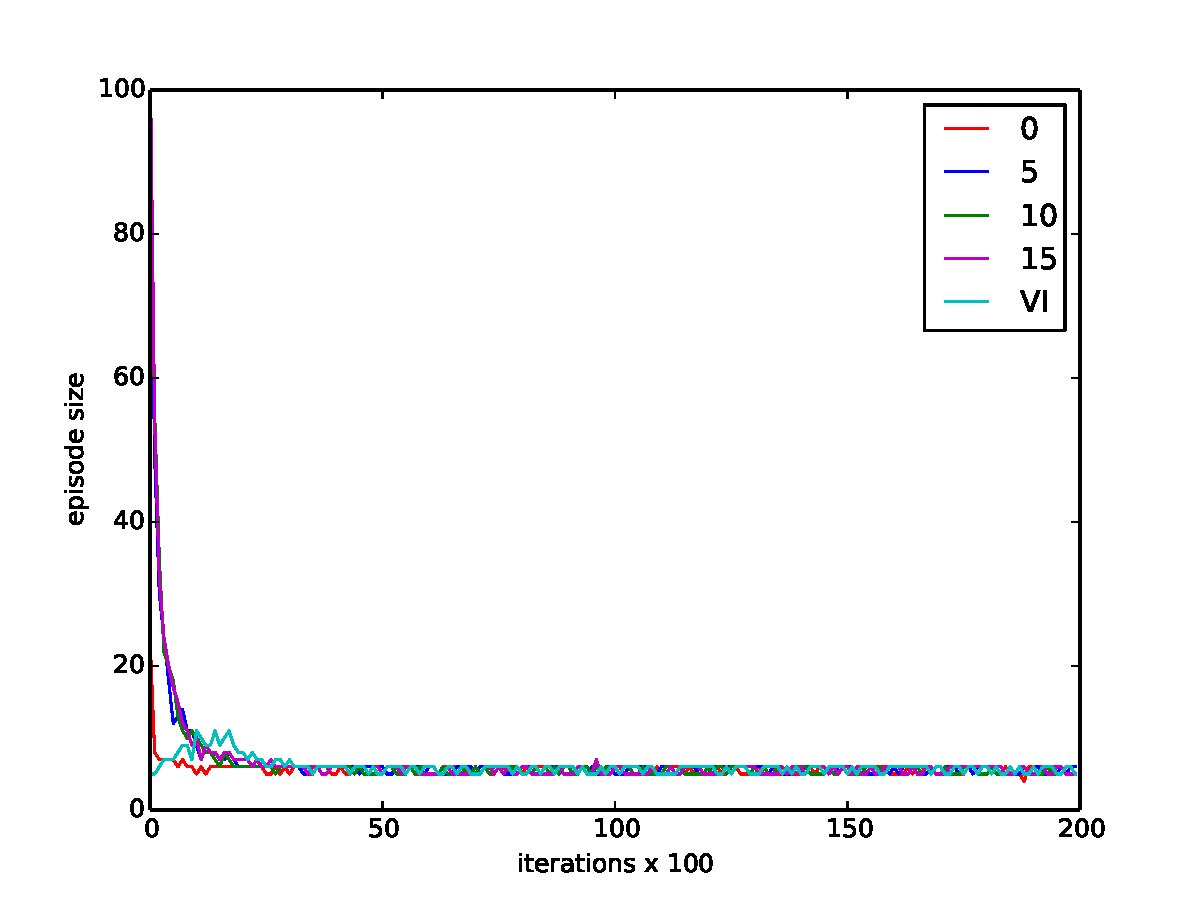
\includegraphics[scale=0.5]{optiInitOverview.pdf}
\caption{Convergence and divergence overview for variable optimistic initialization.} 
\label{figure:optimisticOverview}
\end{figure}
\begin{figure}[H] \centering
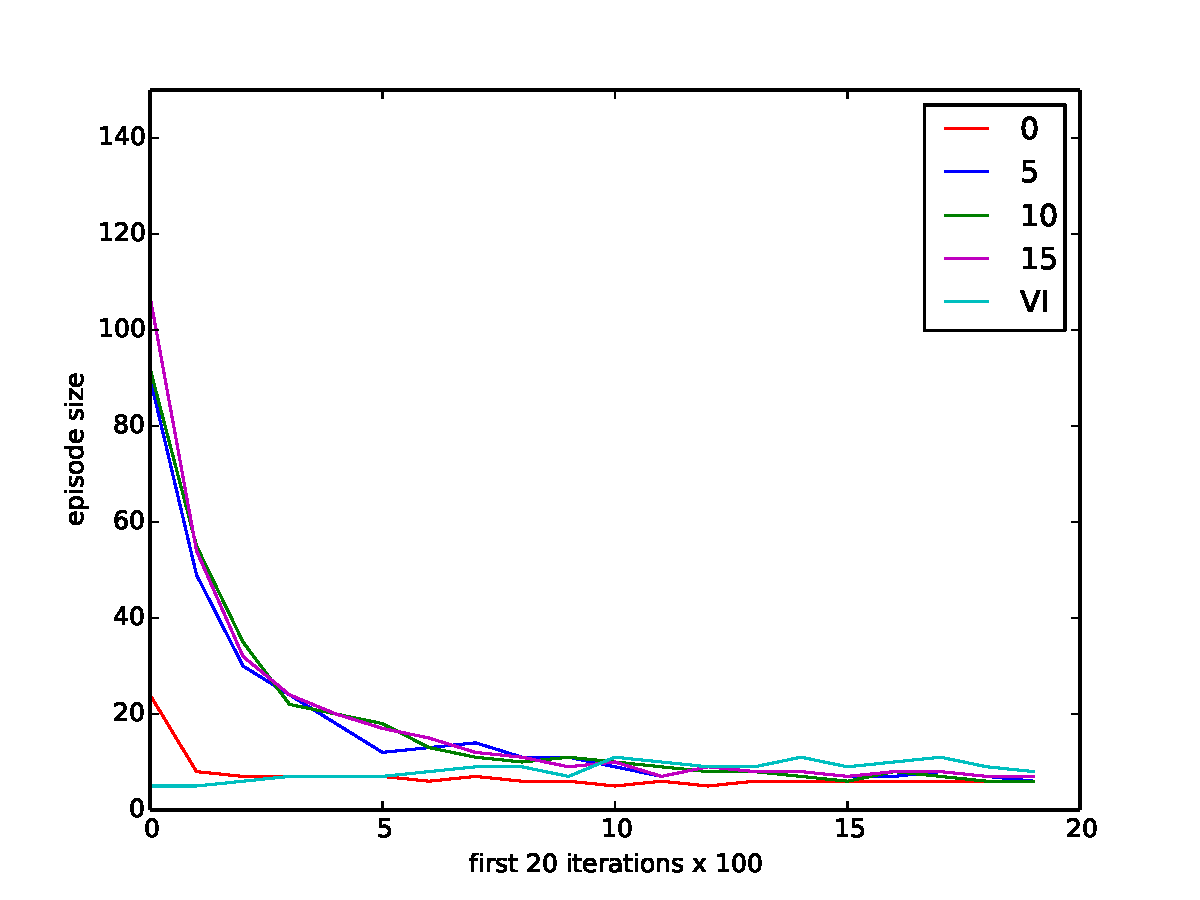
\includegraphics[scale=0.5]{optiInitfirst20x100.pdf}
\caption{Convergence and divergence for variable optimistic initialization in the initial 2000 runs.} 
\label{figure:optimisticfirst20}
\end{figure}
\begin{figure}[H] \centering
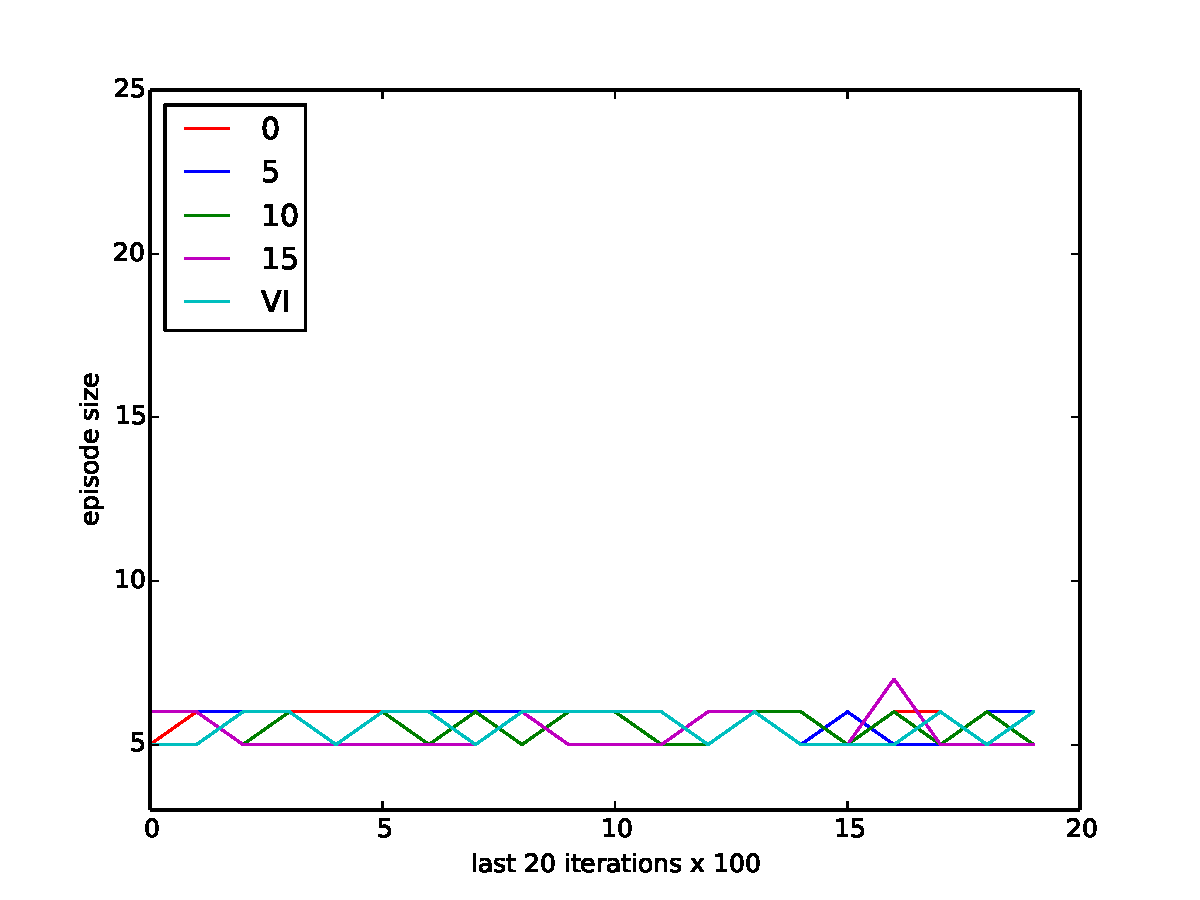
\includegraphics[scale=0.5]{optiInitlast20x100.pdf}
\caption{Convergence for variable optimistic initialization in the last 2000 runs.} 
\label{figure:optimisticlast20}
\end{figure}
\begin{figure}[H] \centering
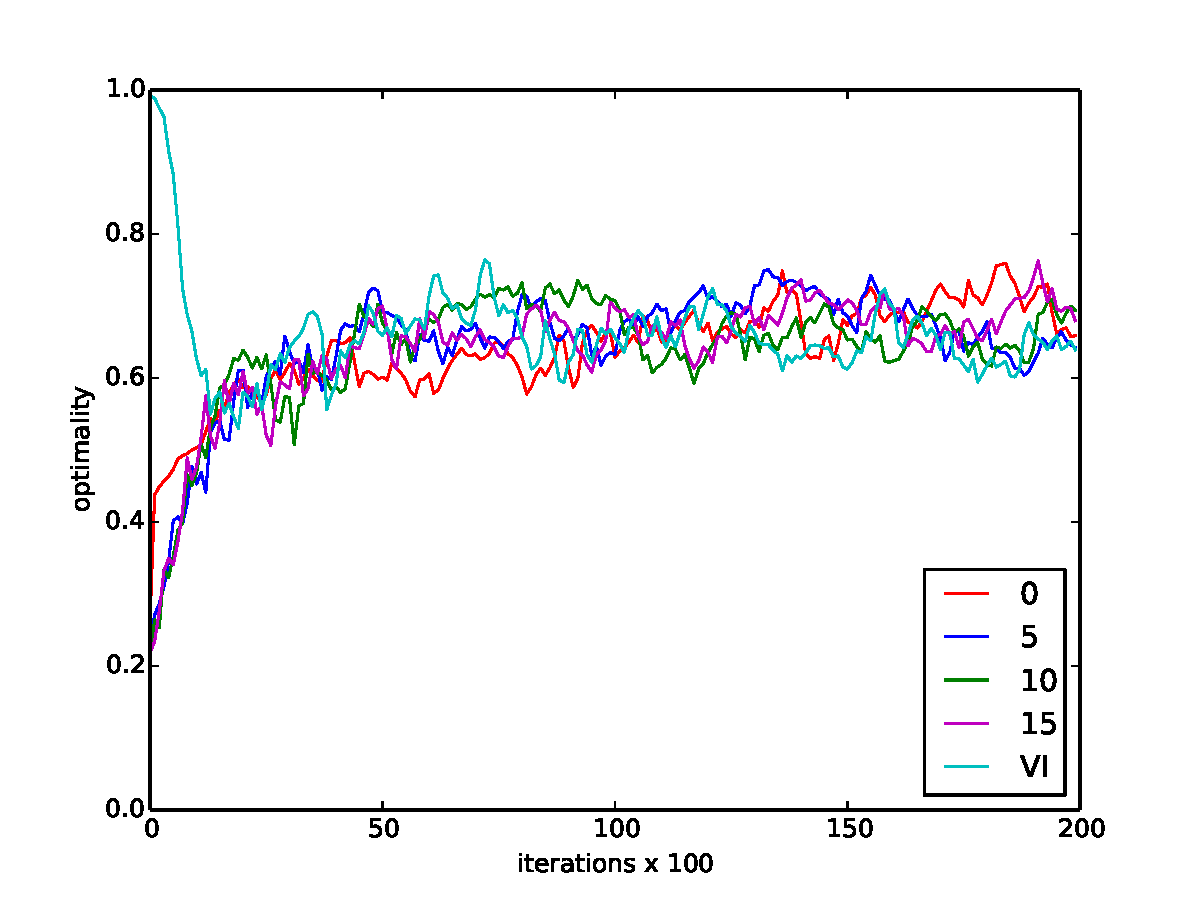
\includegraphics[scale=0.6]{optimalityOptimistic.pdf}
\caption{Divergence from the optimal policy after optimal initialization in case of VI.} 
\label{figure:optiOpti}
\end{figure}
Results for the optimal policy initialization are not surprising, as it confirms our earlier notion that fixed exploration by its parameters will not allow the algorithm to converge back to its optimal policy. We see a sharp drop in its optimality and climbing initial average capture times, due to its straying from the aforementioned. In the end its performance is comparable to the other initialization values and reaches a certain equilibrium governed by the parameters of $\alpha$, $\epsilon$ and $\gamma$. 

In the initialization value of 0 it's interesting to see that the relatively large difference from the maximum reward of 10, allows it to converge a lot faster in comparison to the other initialization values, but quickly loses that advantage when the difference in the value of initialization and maximum reward become smaller. It seems that greediness can also be achieved by an initialization of values with a large $\delta$ from the reward.

\subsection{Q-learning with Softmax action selection: experiments on $\tau$ and comparison with $\epsilon$-greedy}
As in $\epsilon$ for $\espilon$-greedy $\tau$ (temperature) governs the rate of exploration. High temperatures cause the actions to be all (nearly) equiprobable and low temperatures cause a greater difference in selection probability. When $\tau$ reaches 0 in the limit, the action selection becomes the same as greedy action selection. The difference with $\epsilon$-greedy is that it varies the action probabilities as a graded function of the estimated value, where as the aforementioned chooses equally among all actions when in exploring mode. With this notion we expect Softmax to "degrade" more gracefully than $\epsilon$-greedy. Experiments on $\tau$ are done with values of $0.1, 1 \times 10^{-2}, 1 \times 10^{-3}, 1 \times 10^{-4}$ and $1 \times 10^{-5}$, in the following experimental setup:
\begin{table}[H]
\caption{Experimental setup for testing $\tau$}
\centering
\begin{tabular}{|l|r|}
\hline
Parameters & Value \\\hline
$\gamma$ & 0.1 \\\hline
initial Q & 15 \\\hline
$\alpha$ & 0.2\\\hline
$N$ runs & 20000\\\hline
\end{tabular}
\label{expSetupSoftmax}
\end{table}
We compare the results with $\epsilon$-greedy with the same setup as in Table \ref{expSetupSoftmax} and a fixed value of 0.1 for $\epsilon$:
\begin{figure}[H] \centering
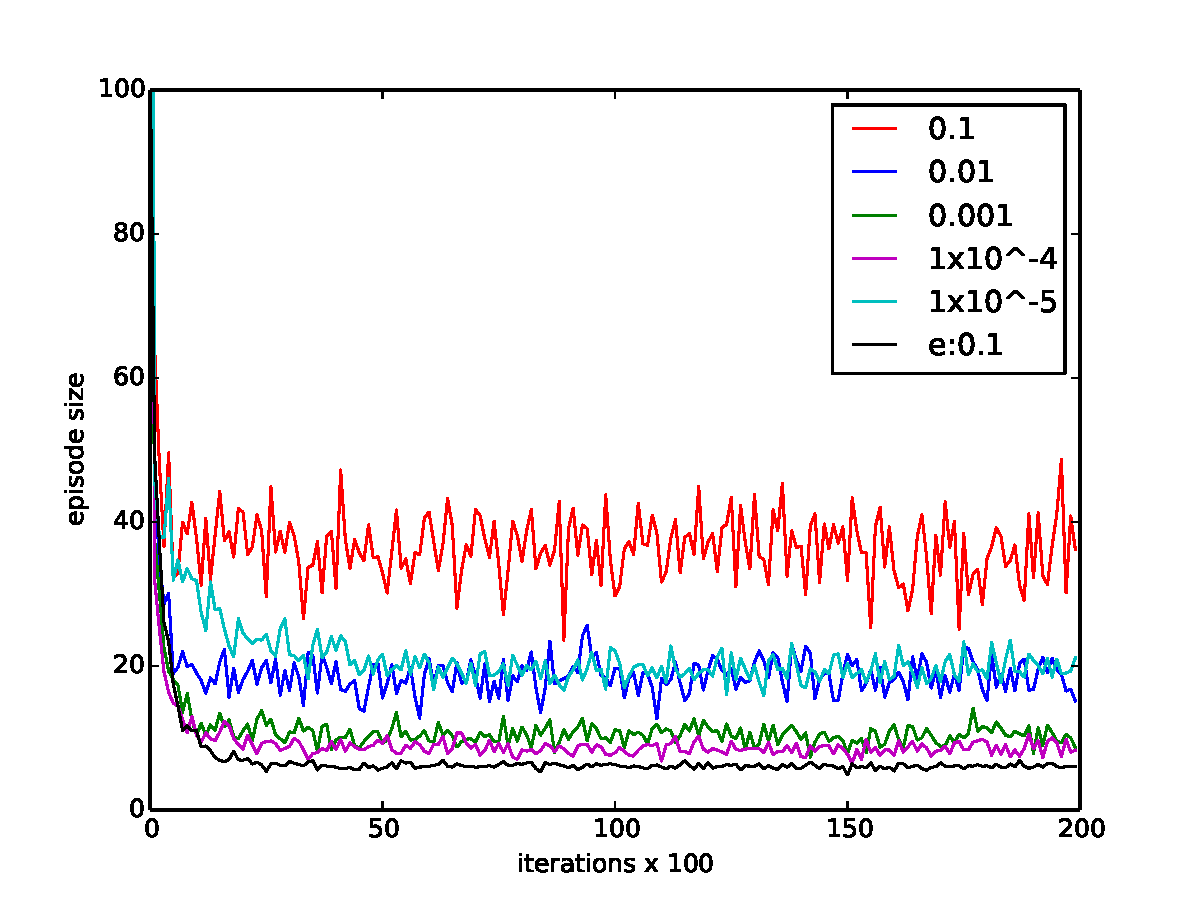
\includegraphics[scale=0.5]{softmaxOverview.pdf}
\caption{Convergence overview for different values of $\tau$ in comparison to $\epsilon$-greedy.} 
\label{figure:softmaxOverview}
\end{figure}
\begin{figure}[H] \centering
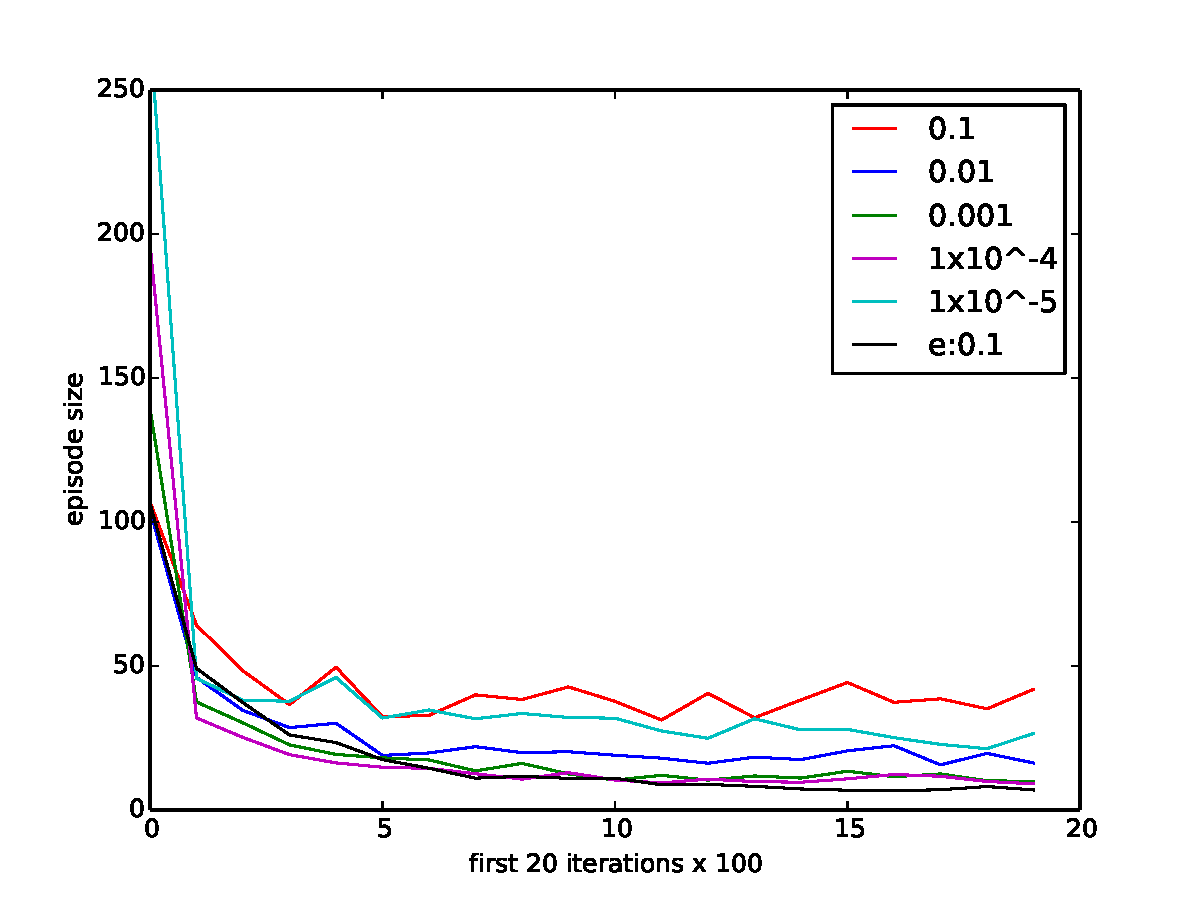
\includegraphics[scale=0.5]{softmaxfirst20x100.pdf}
\caption{Convergence for different values of $\tau$ in the initial 2000 runs in comparison to $\epsilon$-greedy.} 
\label{figure:softmaxfirst20}
\end{figure}
\begin{figure}[H] \centering
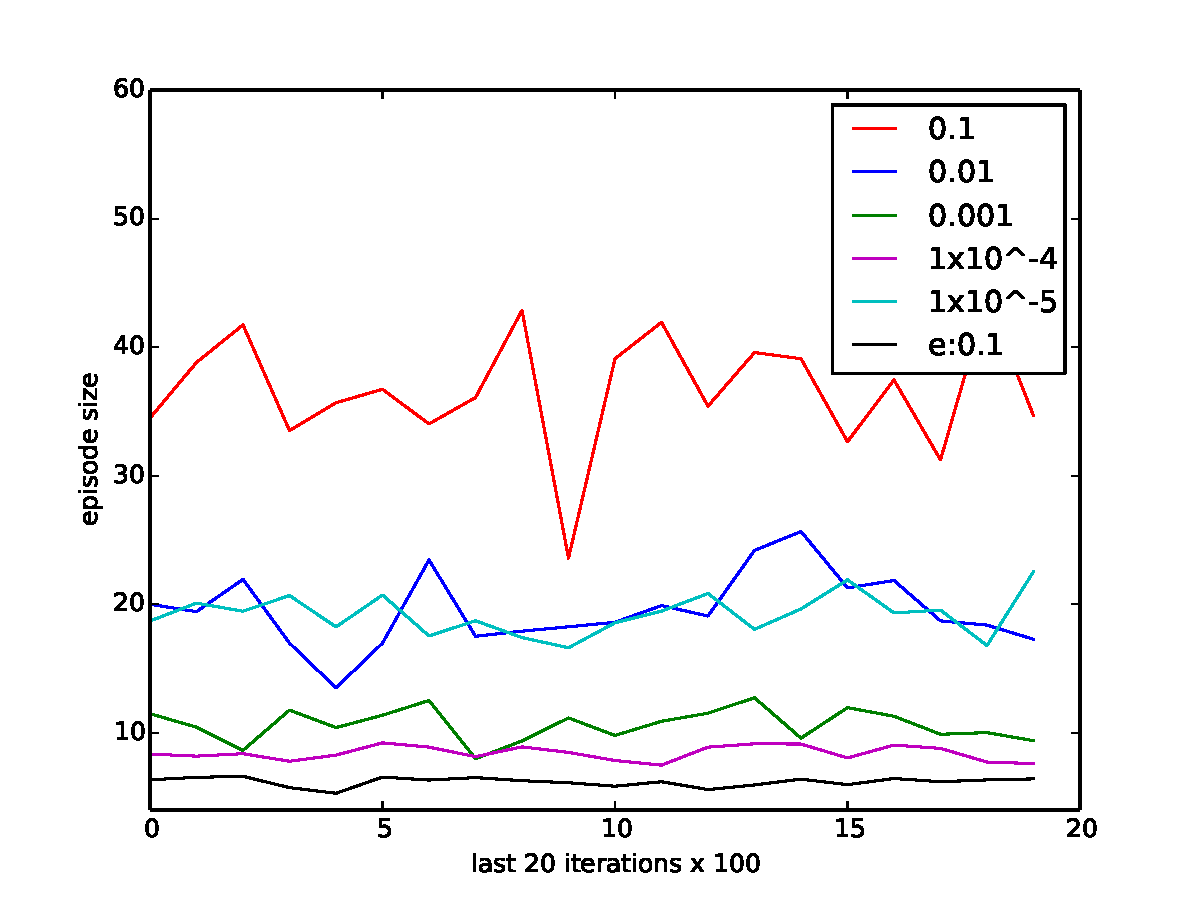
\includegraphics[scale=0.5]{softmaxlast20x100.pdf}
\caption{Convergence for different values of $\tau$ in the last 2000 runs in comparison to $\epsilon$-greedy.} 
\label{figure:softmaxlast20}
\end{figure}
\begin{figure}[H] \centering
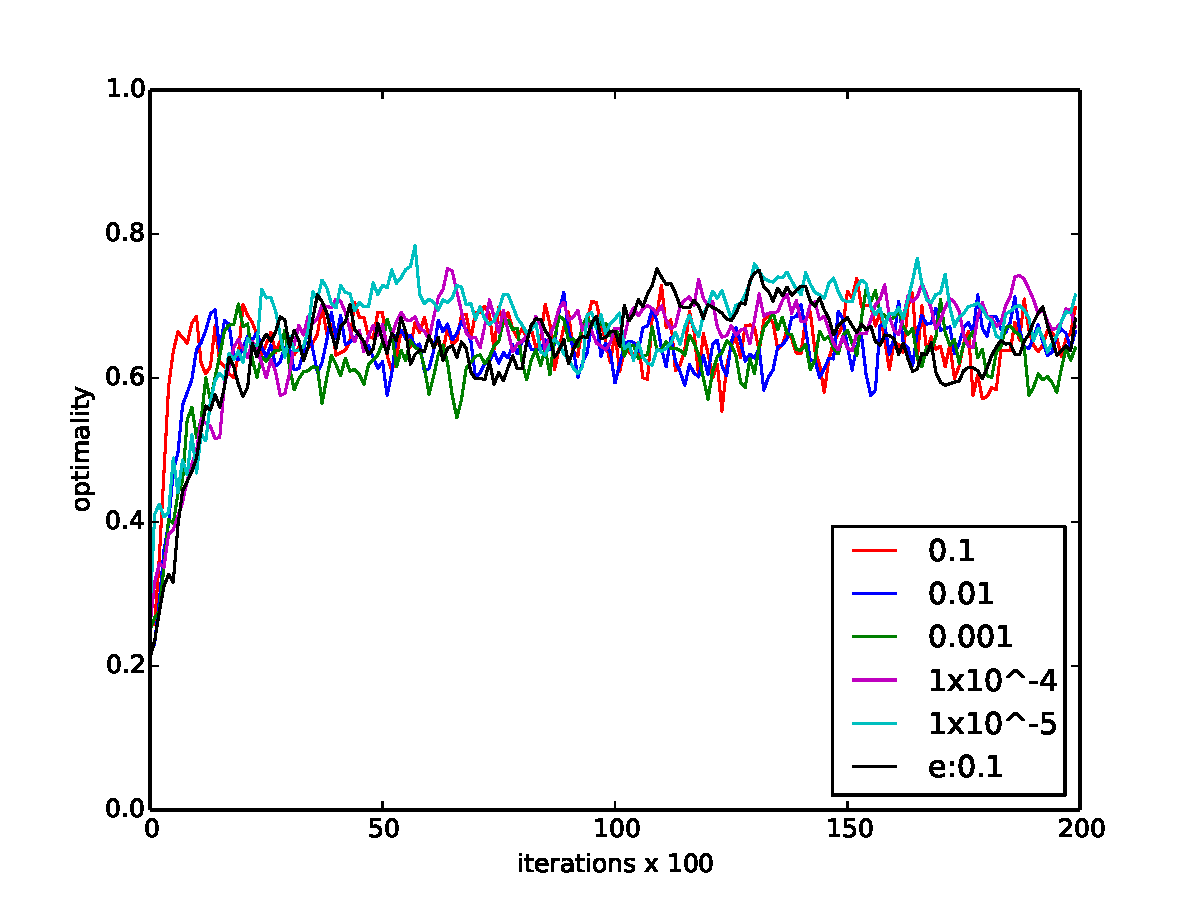
\includegraphics[scale=0.6]{softmaxOptimality.pdf}
\caption{Optimality for different values of $\tau$ as a ratio to the optimal policy in comparison to $\epsilon$-greedy.} 
\label{figure:softmxOpti}
\end{figure}
From the results we see that Softmax has similar behavior to $\epsilon$ when its parameters are high valued. High temperatures favor exploration and give a very fast climb to optimality, but due to the fixation of the parameters, it's "stuck" in exploration mode and its policy is highly fluctuating with an fluctuating high average capture time as a consequence. As in the case of $\epsilon$-greedy would a discounted $\tau$, inverse proportional to the run sequences, benefit further convergence.

In answering the graceful deterioration, we plot different values of $\tau$ against $\epsilon$-greedy with aforementioned parameters in the experimental setup after initialization with the optimal policy, see Figure \ref{figure:softmxGrace}. We can see that while these values of $\tau$ didn't outperform in the average capture times with initialization of 15, see Figure \ref{figure:softmaxOverview}, they do show a much more graceful degradation in its optimality:
\begin{figure}[H] \centering
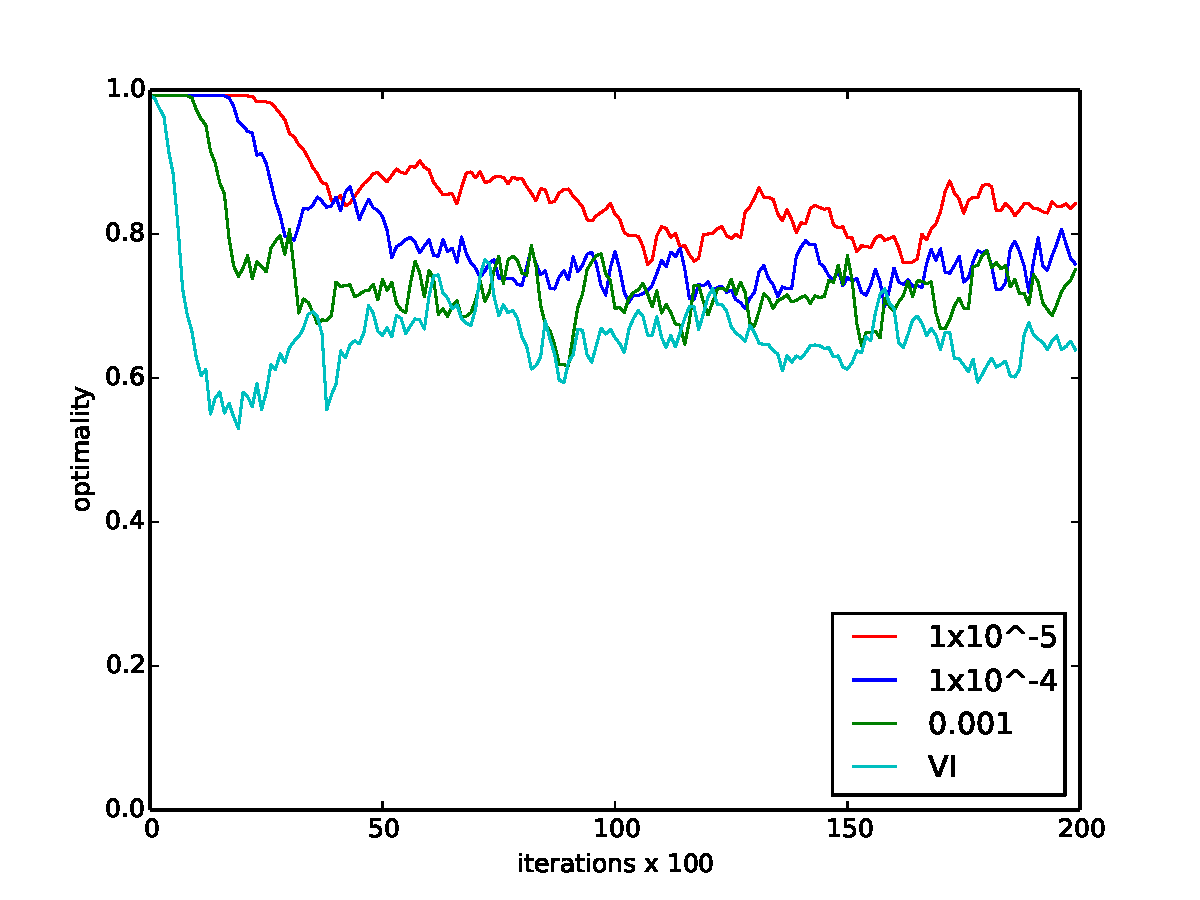
\includegraphics[scale=0.6]{softmaxGrace.pdf}
\caption{Deterioration from the optimal policy for different values of $\tau$ in comparison to $\epsilon$-greedy.} 
\label{figure:softmxGrace}
\end{figure}

\subsection{Sarsa: a comparison with Q-learning in $\epsilon$-greedy and Softmax action selection}
The main difference between Sarsa and Q-learning is that Sarsa being an on-policy method, actually follows the policy being taken and updates its value in respect to that transition. Q-learning, however is directly approximating the optimal policy, regardless of the policy being followed. With this notion we expect Sarsa to converge slower than Q-learning. We'll try to reflect this by plotting comparisons graphs for Q-learning and Sarsa, both with Softmax and $\epsilon$-greedy action selection. The experimental setup is as follow:
\begin{table}[H]
\caption{Experimental setup for Sarsa and Q-learning comparisons.}
\centering
\begin{tabular}{|l|r|}
\hline
Parameters & Value \\\hline
$\gamma$ & 0.1 \\\hline
initial Q & 15 \\\hline
$\alpha$ & 0.2\\\hline
$\epsilon$ & 0.1\\\hline
$\tau$ & $1 \times 10^{-4}$\\\hline
$N$ runs & 20000\\\hline
\end{tabular}
\label{expSetupSarsa}
\end{table}
\begin{figure}[H] \centering
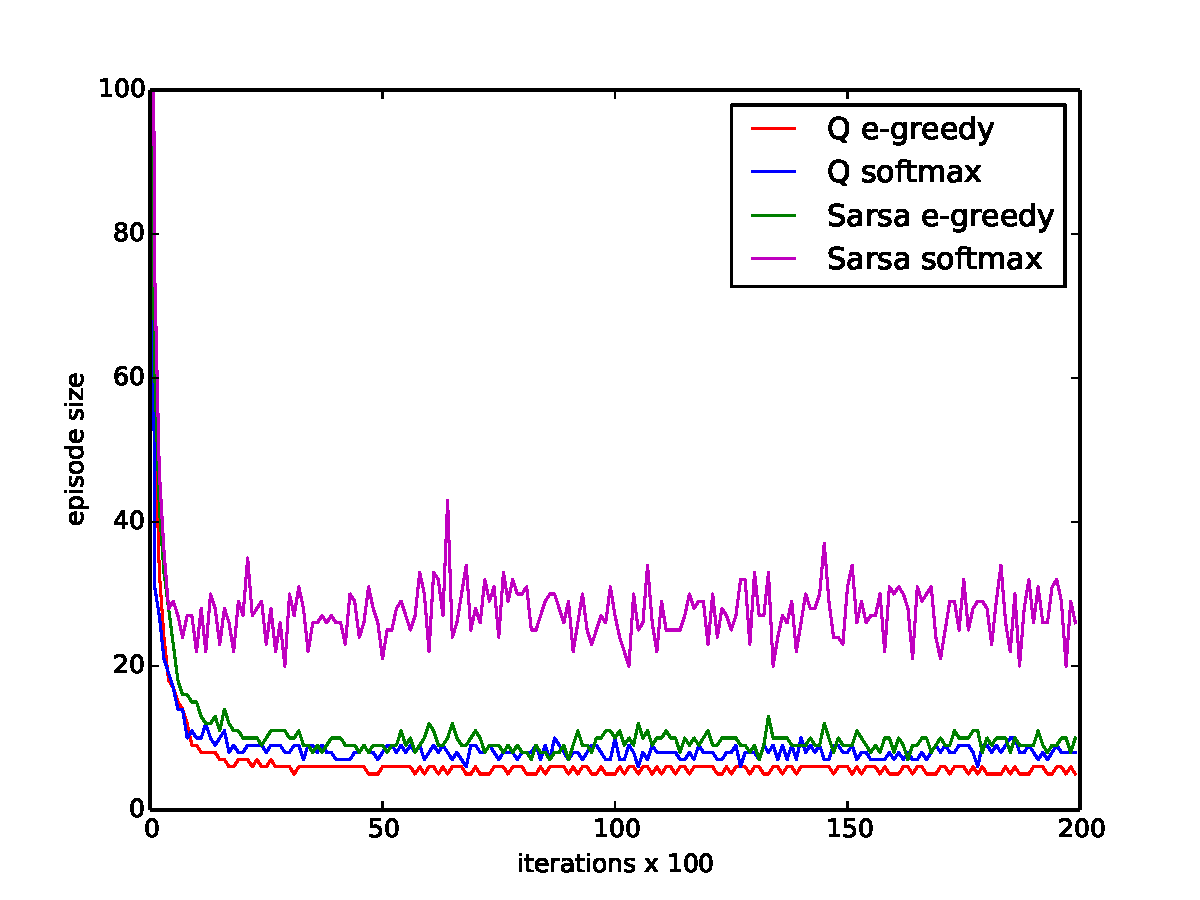
\includegraphics[scale=0.5]{sarsaOverview.pdf}
\caption{Convergence overview for Sarsa and Q-learning in $\epsilon$-greedy and Softmax action selection.} 
\label{figure:sarsaOverview}
\end{figure}
\begin{figure}[H] \centering
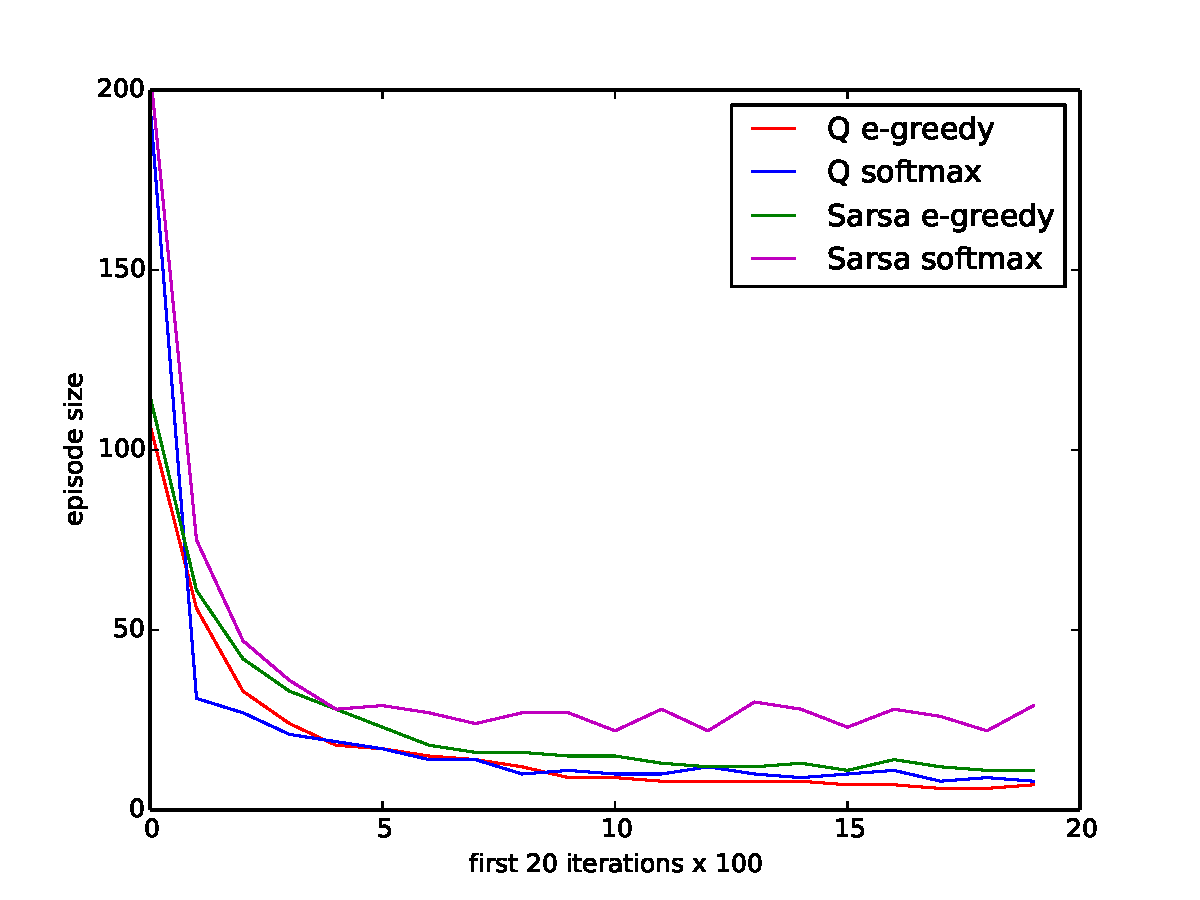
\includegraphics[scale=0.5]{sarsafirst20x100.pdf}
\caption{Convergence for Sarsa and Q-learning in $\epsilon$-greedy and Softmax action selection in the initial 2000 runs.} 
\label{figure:sarsafirst20}
\end{figure}
\begin{figure}[H] \centering
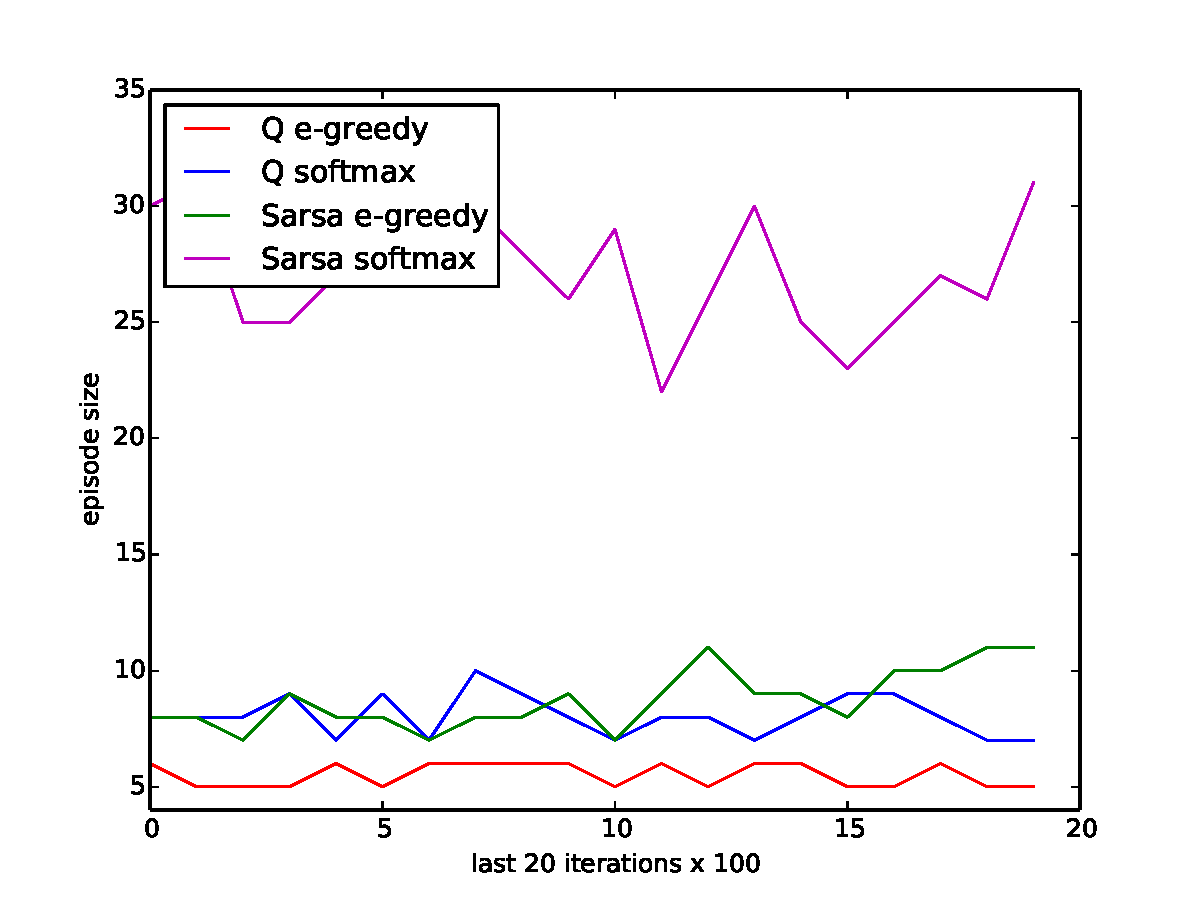
\includegraphics[scale=0.5]{sarsalast20x100.pdf}
\caption{Convergence for Sarsa and Q-learning in $\epsilon$-greedy and Softmax action selection in the last 2000 runs.} 
\label{figure:sarsalast20}
\end{figure}
\begin{figure}[H] \centering
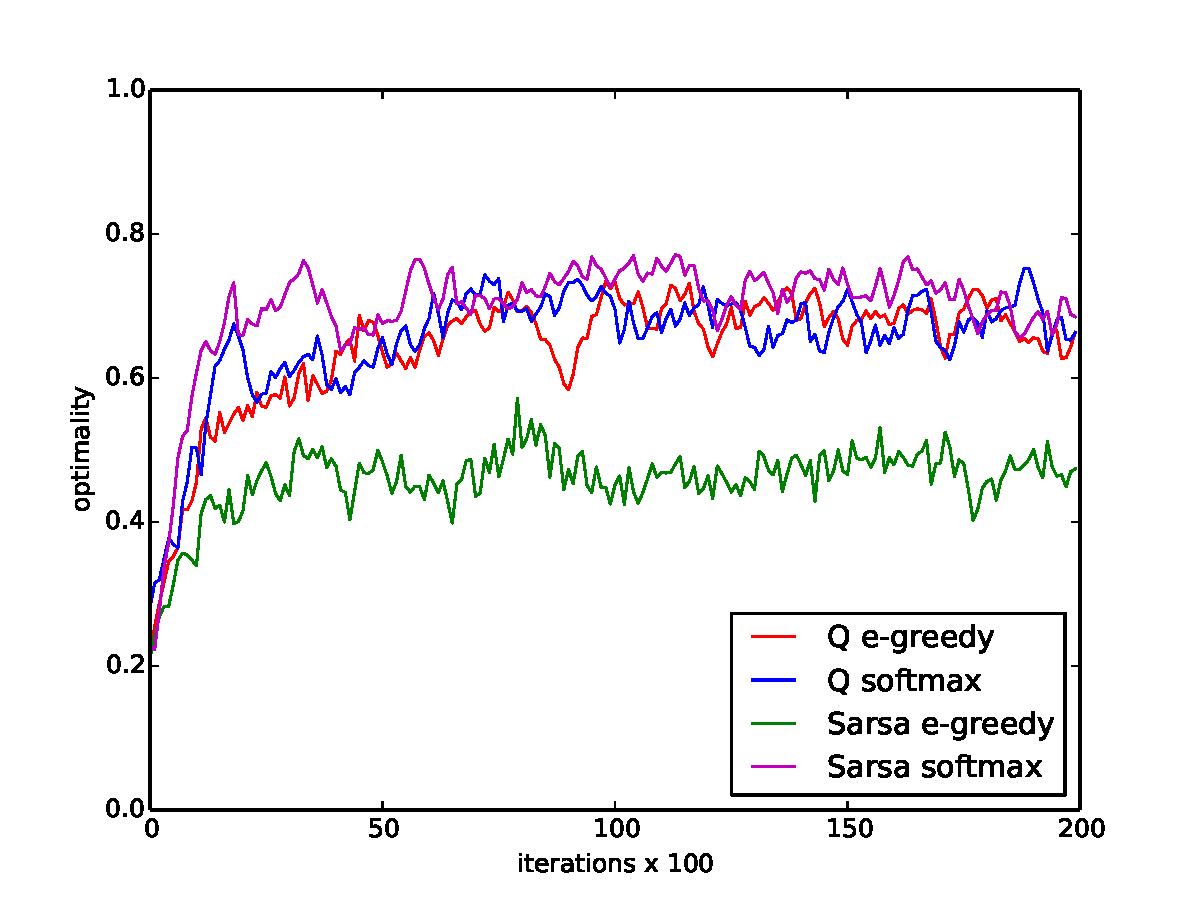
\includegraphics[scale=0.6]{sarsaOptimality.pdf}
\caption{Optimality for for Sarsa and Q-learning in $\epsilon$-greedy and Softmax action selection as a ratio to the optimal policy.} 
\label{figure:sarsaOpti}
\end{figure}
From the results we can see that Sarsa indeed converge slower than its counterpart in Q-learning. Softmax action selection with Sarsa seems to increase its  tendency to explore. We see highly fluctuating high average run times, comparable to Q-learning with large valued $\epsilon$ with $\epsilon$-greedy or even that of large temperature $\tau$ with Softmax, see earlier Figures, while its value here is actually small, $1 \times 10^{-4}$. This exploration mode does favor a fast  convergence to the optimal policy, yet it is not following it, being hindered by its tendency to explore.

\subsection{On-Policy Monte Carlo Control}
By performing this experiment the goal was to see the performance of the On-policy Monte Carlo control in the predator prey environment. The maximum number of control iterations was fixed at $20000$ for every run with different parameters. Additionally the final outcome of the optimal policy was recorded as well as the final values of the function $Q(s,a)$. The metric used in order to determine the performance between different approaches has the size of the episode that was generated each time in the algorithm. A smaller size, between $[1,15]$, shows that the predator catches the prey faster, whereas a bigger size denotes the opposite. Different values for the $\epsilon$ parameter for the $\epsilon$-soft policy were tested, since $\epsilon$ directly influences the amount of exploring and exploiting the agent performs. Additionally, we also experimented on runs with optimistic initial values, namely $15$, for the state-action function $Q(s,a)$, since it also influences the amount of exploration. Only fixed $\epsilon$ values were tested with optimistic initial values of $Q(s,a)$ since they performed better than the adaptive ones, as we will see in the following section. The discount rate $\gamma$ for the returns, was fixed at 0.8.


\subsubsection*{Experiment with different values of $\epsilon$}
The values that we tested were fixed $\epsilon$ at 0.7, 0.5, 0.3, and 0.1, as well as adaptive $\epsilon$ that decreases by $20\%$ every 100 iterations, with different initial value. The results are shown in figure $\ref{figure:differentFixEpsilonOn}$ below. The total number of iterations is  20000, where we take the average episode size every 100 episodes, in order for the visualization to be clearer. 
\begin{figure}[h] \centering
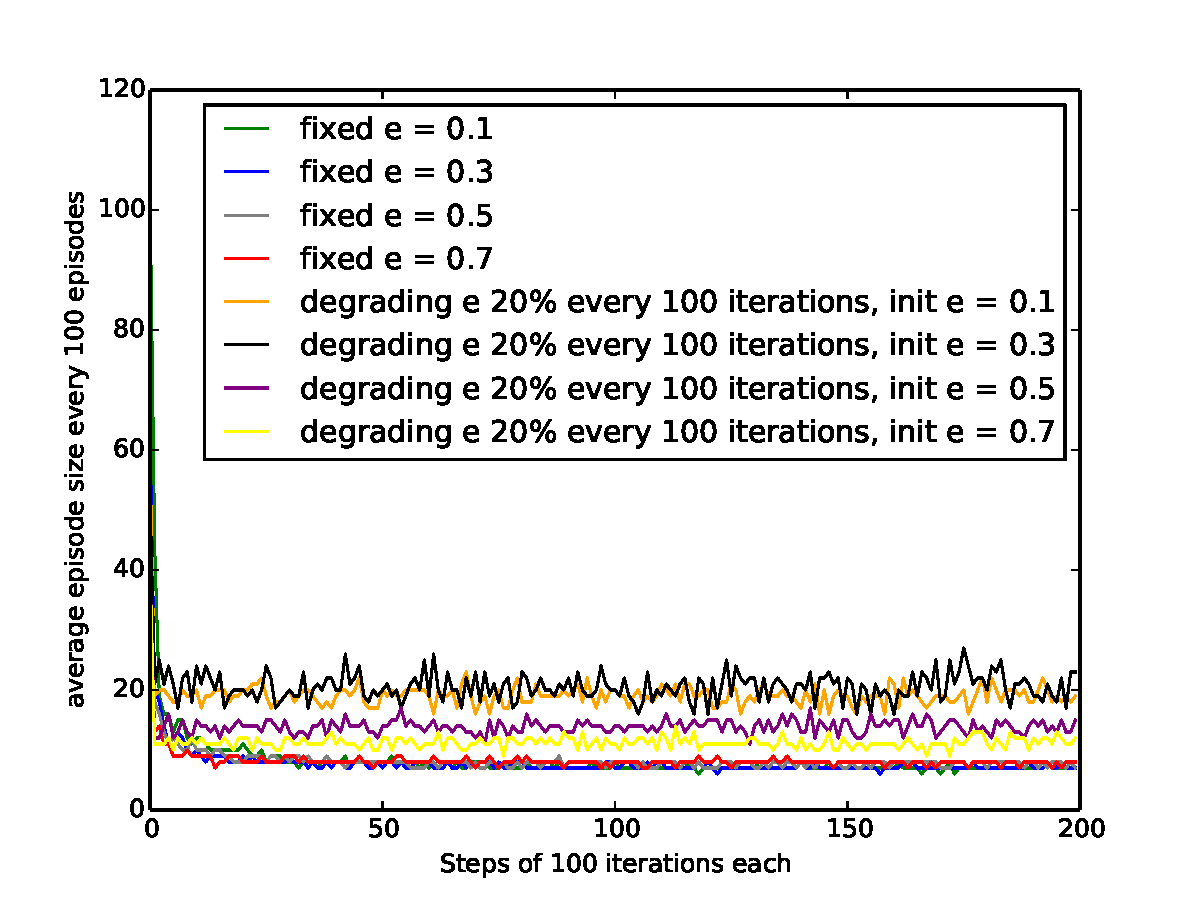
\includegraphics[scale=0.65]{on_policy_mc.pdf}
\caption{On Policy MC catching time with different epsilon value} \label{figure:differentFixEpsilonOn}
\end{figure}

The value of $\epsilon$ directly influences the amount of time it takes for the agent to find a good estimate for the $Q(s,a)$ value. Fixed $\epsilon$ performs better than adaptive $\epsilon$ and this is expected since the degree of exploration is minimized as the number of iterations increases. The effect becomes worser when the initial value of $\epsilon$ is turning lower, since the degree of exploration is limited quite early, hence the agent cannot explore and get a better estimate for the $Q$ value. However higher values allow more exploring, thus getting better results. Fixed $\epsilon$ achieves higher performance since the ratio of exploration/exploitation is consistenly kept during all the control iterations, essentially making the agent explore even in later iterations of the control loop.  We can see from~\ref{figure:differentFixEpsilonOn} that higher  values of $\epsilon$ achieve a sharper decrease in the episode size in the beginning, since there is a bigger episode size which derives from the high exploration probability, but they perform worse in later iterations since they don't exploit as much as lower values of $\epsilon$. The overal best choice seems to be a fixed $\epsilon$ of $0.1$ since it might converge slower to a better policy, but it produces more consistent results in the later iterations, due to the increased rate of exploitation. 

\subsubsection*{Experiment with optimistic initial value of $Q(s,a)$}
Having an optimistic initial value of $Q$ just forces the agent to explore in the begining which creates episodes with an extremely big size, which results in a sharper drop after that since the Q values have a reasonable value again. This approach didn't provide better results though since the estimated values were not obtained through episodes of a reasonable size, hence they were not very accurate. The results can be seen in figure~\ref{figure:differentFixEpsilonOnOpt} where we performed an average of the episode size for every 100 iterations again, in order to produce a clearer visualization.
\begin{figure}[h] \centering
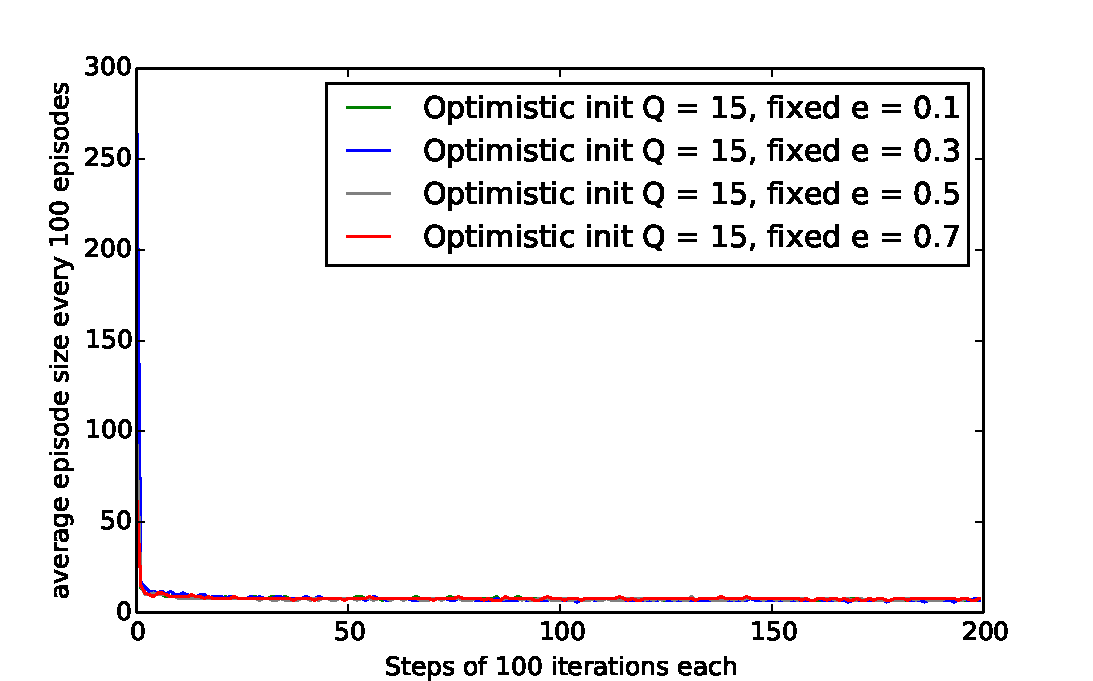
\includegraphics[scale=0.65]{optQOnpolicy.pdf}
\caption{On Policy MC catching time with optimistic initial Q value} \label{figure:differentFixEpsilonOnOpt}
\end{figure}

\subsubsection*{Convergence}
As we have seen in figure~\ref{figure:differentFixEpsilonOn} the algorithm seems to converge in an optimal policy in about $100*100 = 10000$ iterations, which explains the consistent low episode size and faster catch times for the predator. The optimal policy table derived with the best choice of epsilon is shown in~\ref{table:onpolicy} and the $Q(s,a)$ values that the policy was derived from are show in table~\ref{table:valueFunctionOn}. The values are reasonable since they follow the pattern which implies that the further away the predator is from the prey, then the lower the value will be.
\begin{table}[H]
\caption{Target Policy Off-Policy Monte Carlo Control}
\centering
\begin{tabular}{l|l*{9}{c}r}
  \hline
 & 0 & 1 & 2 & 3 & 4 & 5 & 6 & 7 & 8 & 9 & 10 \\ \hline 
0&$\rightarrow$& $\downarrow$&	$\downarrow$&	$\rightarrow$&	$\downarrow$&	$\downarrow$&	$\downarrow$&	$\leftarrow$&	$\downarrow$&	$\leftarrow$&	$\downarrow$	\\
1&$\downarrow$&	$\rightarrow$&	$\downarrow$&	$\rightarrow$&	$\downarrow$&	$\downarrow$&	$\downarrow$&	$\downarrow$&	$\leftarrow$&	$\leftarrow$&	$\downarrow$\\	
2&$\rightarrow$&	$\rightarrow$&	$\rightarrow$&	$\rightarrow$&	$\rightarrow$&	$\downarrow$&	$\leftarrow$&	$\leftarrow$&	$\downarrow$&	$\downarrow$&	$\leftarrow$\\
3&$\rightarrow$&	$\rightarrow$&	$\rightarrow$&	$\rightarrow$&	$\rightarrow$&	$\downarrow$&	$\leftarrow$&	$\leftarrow$&	$\downarrow$&	$\leftarrow$&	$\leftarrow$	\\
4&$\rightarrow$&	$\rightarrow$&	$\rightarrow$&	$\rightarrow$&	$\rightarrow$&	$\downarrow$&	$\leftarrow$&	$\leftarrow$&	$\leftarrow$&	$\leftarrow$&	$\uparrow$\\
5&$\uparrow$&	$\uparrow$&	$\rightarrow$&	$\rightarrow$&	$\rightarrow$&	$P$&	$\leftarrow$&	$\leftarrow$&	$\leftarrow$&	$\uparrow$&	$\rightarrow$	\\
6&$\uparrow$&	$\downarrow$&	$\rightarrow$&	$\uparrow$&	$\uparrow$&	$\uparrow$&	$\leftarrow$&	$\leftarrow$&	$\downarrow$&	$\downarrow$&	$\uparrow$\\	
7&$\rightarrow$&	$\rightarrow$&	$\uparrow$&	$\uparrow$&	$\rightarrow$&	$\uparrow$&	$\leftarrow$&	$\leftarrow$&	$\downarrow$&	$\leftarrow$&	$\leftarrow$\\
8&$\leftarrow$&	$\rightarrow$&	$\rightarrow$&	$\leftarrow$&	$\rightarrow$&	$\uparrow$& $\leftarrow$& $\uparrow$&	$\uparrow$&	$\uparrow$&	$\leftarrow$\\
9&$\uparrow$&	$\uparrow$&	$\downarrow$&	$\rightarrow$&	$\uparrow$&	$\uparrow$&	$\leftarrow$&	$\downarrow$&	$\uparrow$&	$\uparrow$&	$\uparrow$\\
10&$\leftarrow$&	$\rightarrow$&	$\rightarrow$&	$\downarrow$&	$\downarrow$&	$\uparrow$&	$\uparrow$&	$\leftarrow$&	$\leftarrow$&	$\uparrow$&	$\uparrow$\\
\end{tabular}
\label{table:onpolicy}
\end{table}

\begin{table}[H]
\caption{Optimal state value function for each state given prey at (5,5)}
\centering
\begin{tabular}{l|l*{9}{c}r}
  \hline
 & 0 & 1 & 2 & 3 & 4 & 5 & 6 & 7 & 8 & 9 & 10 \\ \hline 
0&1.013 & 1.466 & 1.659 & 2.305 & 2.934 & 3.626 & 2.935 & 2.368 & 1.861 & 1.576 & 1.245 \\
1&1.386 & 1.898 & 2.229 & 2.922 & 3.681 & 4.589 & 3.731 & 2.906 & 2.340 & 1.752 & 1.549 \\
2&1.939 & 2.421 & 2.946 & 3.666 & 4.599 & 5.904 & 4.588 & 3.657 & 3.028 & 1.864 & 1.855 \\
3&1.832 & 2.494 & 3.138 & 4.734 & 5.880 & 7.545 & 5.882 & 4.669 & 3.737 & 2.593 & 2.038 \\
4&2.922 & 3.805 & 4.873 & 6.069 & 7.489 & 10.000 & 7.551 & 6.054 & 4.814 & 3.744 & 1.985\\ 
5&1.785 & 2.977 & 5.805 & 7.533 & 10.000 & 0.000 & 10.000 & 6.836 & 5.345 & 2.817 & 1.902 \\ 
6&1.237 & 2.008 & 4.417 & 5.889 & 6.917 & 10.000 & 7.489 & 6.030 & 2.870 & 2.188 & 1.518 \\
7&2.354 & 3.050 & 3.710 & 4.843 & 5.984 & 7.452 & 5.705 & 4.581 & 2.119 & 2.756 & 1.972 \\
8&1.382 & 1.929 & 2.768 & 1.074 & 4.633 & 5.838 & 4.490 & 3.654 & 2.716 & 2.216 & 1.758 \\
9&1.157 & 1.827 & 1.079 & 2.040 & 1.196 & 4.588 & 2.791 & 1.472 & 2.377 & 1.804 & 1.402 \\
10&0.676 & 1.172 & 1.493 & 1.845 & 2.257 & 3.569 & 2.727 & 2.102 & 1.182 & 0.966 & 0.943 
\end{tabular}
\label{table:valueFunctionOn}
\end{table}


\subsection{Off-Policy Monte Carlo Control}
The purpose of this experiment was to implement Off-Policy Monte Carlo Control algorithm and to observe the results in terms of the target policy, maximum action value function, and also the number of steps the predator take to catch the prey. We tried two different approaches of setting the $\epsilon$ of the behavior policy, fixed value and dynamic value which will be explained in the next part. Different fixed $\epsilon$ value of $\epsilon$-greedy policy also were tested to show how this parameter, which represents the probability of exploring and exploiting, affect the learning processes of action value function. We organize this subsection starting from presenting the results of using different approach of setting $\epsilon$ value of behavior policy, then we show the result of using several different fixed values of $\epsilon$, and finally we will show the convergence of the target policy. 

\subsubsection*{Experiment with different approaches of setting $\epsilon$ value}
Firstly we set the $\epsilon$ value in $\epsilon$-greedy policy as a fix number, then we tried a different approach by making it dynamic by reducing the value after each fix number of iterations. The idea behind this approach was to put more chance in exploration at the beginning and slowly reduced the chance thus it started to exploit more time after time, but also maintained it to be stochastic in order to keep the learning process run.

Figure $\ref{figure:fixEpsilon}$ shows the number of steps the predator took to catch the prey in every iteration governed by the target policy. The $\epsilon$ value was set to be fix of 0.1. In order to get a consistent measurement, the episodes were generated from fix start points of the predator and the prey, which were (0,0) and (5,5) respectively. The time that the predator took to catch the prey can be used to measure the performance of Off-Policy Monte Carlo Learning after each iteration, because the target policy uses the $Q$ value immediately after each iteration. Since the target policy was greedy, then it always take best action based on the $Q$ value. The better the $Q$ value, the better target policy's performance should be.

\begin{figure}[H] \centering
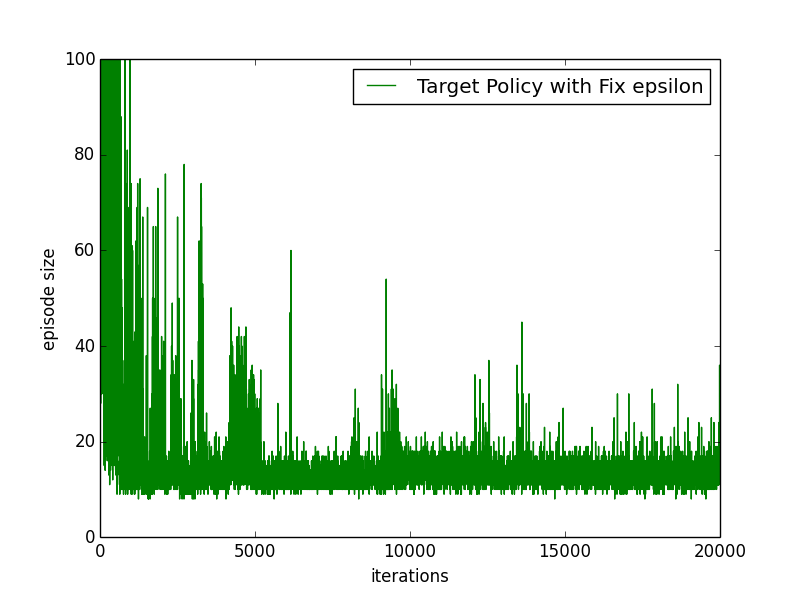
\includegraphics[scale=0.5]{target_fix_0_1.png}
\caption{Catching time with fix epsilon value} \label{figure:fixEpsilon}
\end{figure}

\begin{figure}[H] \centering
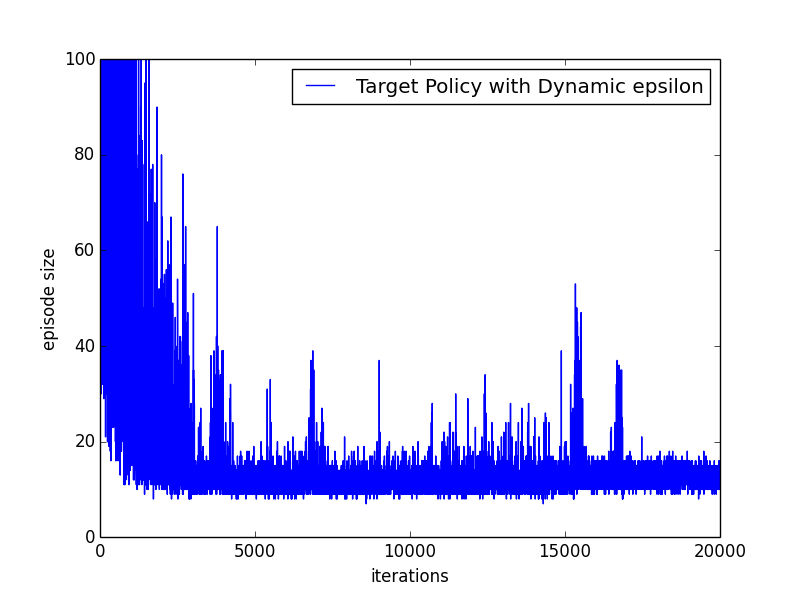
\includegraphics[scale=0.5]{target_dynamic_0_5_0_8_0_05.png}
\caption{Catching time with dynamic epsilon value}\label{figure:dynamicEpsilon} \label{figure:dynamicEpsilon}
\end{figure}

Figure $\ref{figure:dynamicEpsilon}$ was generated from the same setting as before except the value of $\epsilon$ was set to dynamically changed over iteration. First we set the value to 0.5 then after every 500 iterations it was reduced by multiplying with 0.8. In order to maintain the value not become too small, we set the minimum value to 0.1, because if $\epsilon$ is too small then it will become greedy and almost never explore anymore. As a consequence, learning processes will stop because both behavior and target policy always agree on actions taken in the generated episodes.

Even though the difference between the two figures above is not significant, but we can still see the influence of setting the $\epsilon$ value to a fix and to a dynamic value. For fix value approach, the number of time drop quicker than the one from dynamic approach. This is because the fix value approach exploited more even from beginning due to the probability of exploiting much larger than exploring. On the other hand,the dynamic approach give the same probability between exploiting and exploring, so at the beginning it explored more than the fix value approach. Now let us see the last 3000 iterations from the two figures, it can be seen that dynamic value approach shows a slightly better performance, it fluctuates less than that in the other figure. Since the difference is not significant then we can not claim which one is better. The general statement is that they both can converge with anough number of iterations.

%{\raggedleft{}Some text flushed right.}
\subsubsection*{Experiment with different values of $\epsilon$}
In this part we made some experiments by changing the fix value of $\epsilon$. Since the epsilon represents the chance of exploring and exploiting in learning, then we will make a conclusion related to that matter. 

The values that we tested was 0.5, 0.3, 0.1, and 0.001, and the result is shown by figure $\ref{figure:differentFixEpsilon}$ below. The number of iterations is  10000, to make a clearer figure, we devided it into 200 parts, and averaged each part, so 1 iteration in the figure is average of 50 iterations. 
\begin{figure}[H] \centering
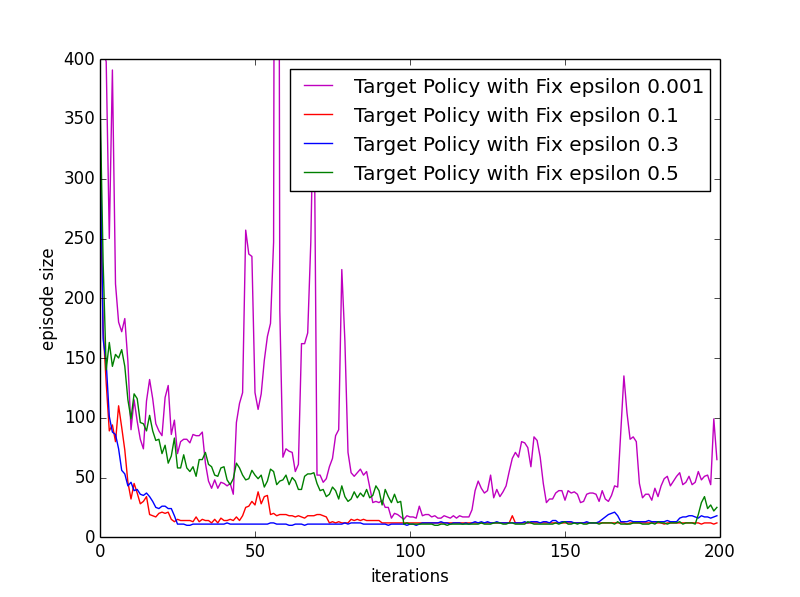
\includegraphics[scale=0.6]{target_fix_different_epsilon4.png}
\caption{Catching time with different fixed epsilon value} \label{figure:differentFixEpsilon}
\end{figure}

The figure above tells us that in our test case, $\epsilon$ value of 0.1 and 0.3 give the best performance, while 0.5 result shows a slower convergence than the previous values and 0.001 become the worst. This result confirm that exploration and exploitation have a significant role in learning process. Setting the exploitation probability value too small makes the model hard to learn, it could be trapped to exploit wrong actions, where setting the value too high means small chance to exploiting and then leads to a late convergence.

\subsubsection*{Convergence}
In this section we will show the convergence of the Off-Policy Monte Carlo Control method. Table $\ref{table:valueFunctionOff}$ and table $\ref{table:TargetPolicyOff}$ show the optimal value function and the optimal target policy's actions respectively. Even though this method use sampling to estimate the target policy, but with enough number of iteration the convergence to the optimal value function can be reach. From several experiments, we know that as long as the behavior policy is stochastic and has reasonable $\epsilon$ value, like what we have explained in the previous part, then it will converge. The results below were generated from 100.000 iterations with fixed $\epsilon$ 0.3.

\begin{table}[H]
\caption{Optimal state value function for each state given prey at (5,5)}
\centering
\begin{tabular}{l|l*{9}{c}r}
  \hline
 & 0 & 1 & 2 & 3 & 4 & 5 & 6 & 7 & 8 & 9 & 10 \\ \hline 
0&1.282 & 1.501 & 2.068 & 2.514 & 3.149 & 3.673 & 2.949 & 2.488 & 2.028 & 1.626 & 1.324 \\
1&1.540 & 2.055 & 2.469 & 3.208 & 3.974 & 4.694 & 3.951 & 3.185 & 2.573 & 2.006 & 1.791 \\
2&1.896 & 2.691 & 3.198 & 3.987 & 4.939 & 6.054 & 4.958 & 3.999 & 3.201 & 2.576 & 1.965 \\
3&2.622 & 3.233 & 3.985 & 4.943 & 6.150 & 7.611 & 6.198 & 4.971 & 4.027 & 3.191 & 2.395 \\
4&3.058 & 4.004 & 4.960 & 6.156 & 7.609 & 10.000 & 7.631 & 6.192 & 4.712 & 3.837 & 2.962\\ 
5&3.763 & 4.738 & 6.005 & 7.633 & 10.000 & 0.000 & 10.000 & 7.616 & 6.026 & 4.729 & 3.721 \\ 
6&3.207 & 3.967 & 4.928 & 6.159 & 7.620 & 10.000 & 7.597 & 5.981 & 4.852 & 3.699 & 3.007 \\
7&2.587 & 3.240 & 4.007 & 4.987 & 6.011 & 7.624 & 6.164 & 4.887 & 3.912 & 3.144 & 2.540 \\
8&2.129 & 2.202 & 3.174 & 4.005 & 4.830 & 6.037 & 4.749 & 3.781 & 3.073 & 2.494 & 2.073 \\
9&1.695 & 2.091 & 2.624 & 3.240 & 3.747 & 4.752 & 3.845 & 2.947 & 2.564 & 2.021 & 1.511 \\
10&1.199 & 1.706 & 1.964 & 2.349 & 2.925 & 3.733 & 3.038 & 2.451 & 1.971 & 1.715 & 1.378 
\end{tabular}
\label{table:valueFunctionOff}
\end{table}

\begin{table}[H]
\caption{Optimal target policy's actions for each state given the prey at (5,5)}
\centering
\begin{tabular}{l|l*{9}{c}r}
  \hline
 & 0 & 1 & 2 & 3 & 4 & 5 & 6 & 7 & 8 & 9 & 10 \\ \hline 
0 & $\rightarrow$&	$\downarrow$&	$\downarrow$&	$\rightarrow$&	$\downarrow$&	$\downarrow$&	$\leftarrow$&	$\leftarrow$&	$\leftarrow$&	$\leftarrow$&	$\leftarrow$\\	
1&$\rightarrow$&	$\rightarrow$&	$\rightarrow$&	$\rightarrow$&	$\downarrow$&	$\downarrow$&	$\leftarrow$&	$\downarrow$&	$\leftarrow$&	$\leftarrow$&	$\leftarrow$	\\
2&$\downarrow$&	$\rightarrow$&	$\downarrow$&	$\rightarrow$&	$\downarrow$&	$\downarrow$&	$\downarrow$&	$\downarrow$&	$\leftarrow$&	$\leftarrow$&	$\downarrow$\\	
3&$\downarrow$	&$\downarrow$&	$\rightarrow$&	$\rightarrow$&	$\downarrow$&	$\downarrow$&	$\leftarrow$&	$\leftarrow$&	$\leftarrow$&	$\downarrow$&	$\downarrow$\\	
4&$\rightarrow$&	$\rightarrow$&	$\rightarrow$&	$\rightarrow$  &	$\downarrow$&	$\downarrow$&	$\downarrow$&	$\downarrow$&	$\downarrow$&	$\leftarrow$&	$\leftarrow$\\	
5&$\rightarrow$  &	$\rightarrow$  &	$\rightarrow$  &	$\rightarrow$ &	$\rightarrow$ &	$P$ &	$\leftarrow$&	$\leftarrow$&	$\leftarrow$&	$\leftarrow$&	$\leftarrow$\\	
6&$\rightarrow$ &	$\rightarrow$ &	$\uparrow$&	$\rightarrow$ &	$\rightarrow$ &	$\uparrow$&	$\leftarrow$&	$\leftarrow$&	$\leftarrow$&	$\uparrow$&	$\leftarrow$\\	
7&$\rightarrow$ &	$\rightarrow$ &	$\rightarrow$ &	$\uparrow$&	$\rightarrow$ &	$\uparrow$&	$\uparrow$&	$\leftarrow$&	$\leftarrow$&	$\leftarrow$&	$\leftarrow$\\	
8&$\uparrow$&	$\rightarrow$ &	$\uparrow$&	$\uparrow$&	$\uparrow$&	$\uparrow$&	$\uparrow$&	$\leftarrow$&	$\leftarrow$&	$\leftarrow$&	$\leftarrow$\\	
9&$\rightarrow$ &	$\uparrow$&	$\uparrow$&	$\rightarrow$ &	$\uparrow$&	$\uparrow$&	$\uparrow$&	$\leftarrow$&	$\leftarrow$&	$\uparrow$&	$\uparrow$\\	
10&$\uparrow$&	$\uparrow$&	$\rightarrow$ &	$\uparrow$&	$\uparrow$&	$\uparrow$&	$\uparrow$&	$\leftarrow$&	$\leftarrow$&	$\leftarrow$&	$\leftarrow$
\end{tabular}
\label{table:TargetPolicyOff}
\end{table}

\subsection{Comparison of all approaches to the learning problem}
Regarding on and off policy Monte Carlo control, in the case of the best parameters $\epsilon$ for both of the algorithms, the On-policy Monte Carlo performs better. It converges faster to an optimal policy that produces faster catch times for the predator and manages to keep them consistent in the later episodes. On the contrary Off-policy seems to converge slower and has some fluctuations on the catch times which was derived from the fact that the optimization of the target policy was done through a different behaviour policy. Furthermore, in the off-policy method, state-action pairs that will be used to estimate are only pairs that occur after the last different action between the two policies. So it is likely to use fewer samples than those in on-policy with the same number of iterations. The average catch times for the last $100$ episodes are shown in table~\ref{compavg} and show the fact that on-policy Monte Carlo produces a better policy.
\begin{figure}[H] \centering
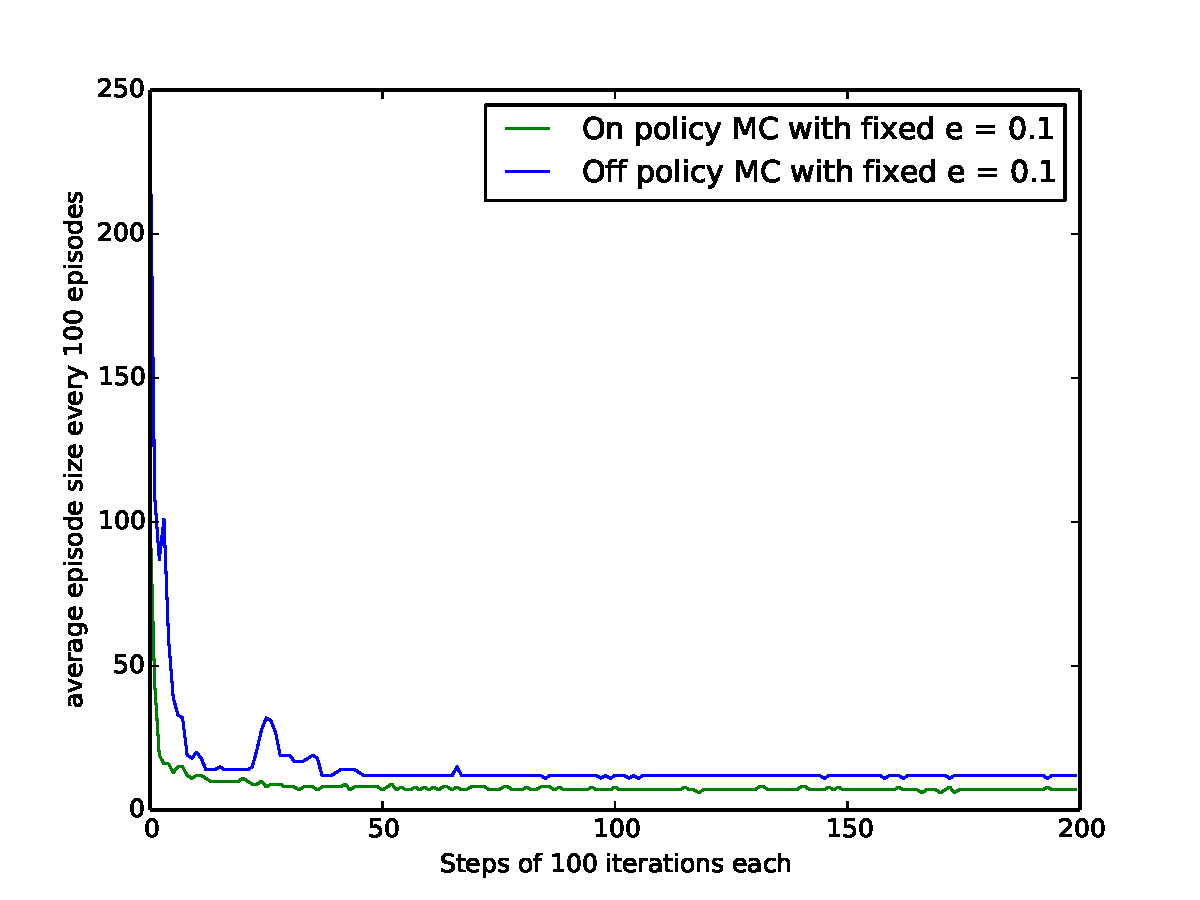
\includegraphics[scale=0.6]{onOffComp.pdf}
\caption{Catching times for best choice of $\epsilon$ for On and Off policy MC}\label{figure:onoffcomp} 
\end{figure}

\begin{table}[H]
\caption{Average catching time for all algorithms at convergence}
\centering
\begin{tabular}{|l|r|}
\hline
Method & Average \\\hline
Q-Learning& 0 \\\hline
Sarsa& 0 \\\hline
On-policy MC& 7\\\hline
Off-policy MC& 12\\\hline
\end{tabular}
\label{compavg}
\end{table}

\section{conclusion}
\label{discussion}
In this research, we have explored the problem of the single agent learning by using different methods that highlight this problem. Monte Carlo methods as well as Temporal-Difference methods have been used, namely On and Off policy Monte Carlo control, Q-Learning and Sarsa.\\
Regarding the on-policy Monte Carlo Control method, we conclude that the optimal policy can be reached quite fast, since the convergence happens in a relative few episodes, and finally the average catching time is low, which is a good indication of an optimal policy.\\
Even though it seems to converge slower than the on-policy, but in most cases, with the stochastic behavior policy and enough number of iterations, the off-policy Monte Carlo method will converge to the optimal policy. In our test case, 0.1 and 0.3 of epsilon value performed best.\\
The advantage of off-policy over on-policy is that the policy that we want to estimate can be greedy, so if we use this policy in the middle of learning, it exactly represents the condition of the value function at that time.



\begin{thebibliography}{9}

\bibitem{suttonBarto}
  Richard S. Sutton, Andrew G. Barto,
  \emph{Reinforcement Learning: An Introduction}.
  MIT Press, Cambridge, MA, 
  A Bradford Book,
  1998.

\end{thebibliography}

%%% End document
\end{document}

